% LEDGER 项目计划书
% 编译：cd paper/proposal && latexmk -xelatex main.tex   （或 bash build.sh）
\documentclass[fontset=none,zihao=5,oneside,openany]{ctexbook}
\usepackage{ledger}
\renewcommand{\chaptermark}[1]{\markboth{#1}{}}

\begin{document}
\frontmatter
% 封面
\thispagestyle{empty}
\begin{tikzpicture}[remember picture,overlay]
  % 账页底
  \fill[paper] (current page.south west) rectangle (current page.north east);
  \foreach \i in {1,...,46}{
    \draw[rule!75,line width=0.25pt] ([yshift=-\i*0.62cm-0.8cm]current page.north west) -- ([yshift=-\i*0.62cm-0.8cm]current page.north east);}
  % 左侧双红线（账簿的页边线）
  \draw[seal,line width=0.7pt] ([xshift=2.6cm]current page.north west) -- ([xshift=2.6cm]current page.south west);
  \draw[seal,line width=0.7pt] ([xshift=2.75cm]current page.north west) -- ([xshift=2.75cm]current page.south west);
  % 顶部墨蓝带
  \fill[ink] (current page.north west) rectangle ([yshift=-3.1cm]current page.north east);
  \node[anchor=west,text=white,font=\heiti\small] at ([xshift=3.3cm,yshift=-1.25cm]current page.north west)
    {2026 北京市大学生金融人工智能竞赛};
  \node[anchor=west,text=white!75,font=\heitilight\footnotesize] at ([xshift=3.3cm,yshift=-1.95cm]current page.north west)
    {竞赛主题：金融投研智能体构建\quad·\quad 初赛提交材料};
  \node[anchor=east,text=white,font=\sffamily\footnotesize\bfseries,align=right] at ([xshift=-1.6cm,yshift=-1.55cm]current page.north east)
    {PROJECT\\PROPOSAL};

  % 主标题
  \node[anchor=north west,inner sep=0pt] at ([xshift=3.3cm,yshift=-6.3cm]current page.north west) {%
    \begin{minipage}{14.2cm}
      {\fontsize{72}{72}\selectfont\rmfamily\color{ink}\addfontfeature{LetterSpace=6}LEDGER\par}
      \vspace{10pt}
      {\color{seal}\rule{3.2cm}{2pt}\par}
      \vspace{10pt}
      {\sffamily\small\color{inkl}\textbf{L}LM-driven \textbf{E}quity Research with \textbf{D}eterministic\\
       \textbf{G}rounding, \textbf{E}valuation and \textbf{R}eporting\par}
      \vspace{1.3cm}
      {\heiti\bfseries\fontsize{25}{34}\selectfont\color{ink}可追溯的 A 股投研多智能体系统\par}
      \vspace{6pt}
      {\heitilight\fontsize{15}{22}\selectfont\color{ink}从一份年报到一份经得起核对的深度研报\par}
      \vspace{1.1cm}
      {\heiti\bfseries\fontsize{17}{22}\selectfont\color{seal}项\,目\,计\,划\,书\par}
    \end{minipage}};

  % 选题标签
  \node[anchor=north west,inner sep=0pt] at ([xshift=3.3cm,yshift=-17.6cm]current page.north west) {%
    \begin{minipage}{14.5cm}\small
      \renewcommand{\arraystretch}{1.5}
      \begin{tabular}{@{}l@{\hspace{1.2em}}l@{}}
        {\heiti\bfseries\color{seal}主选题} & 财报分析\quad·\quad 自动化估值建模\quad·\quad 研究报告质量评估 \\
        {\heiti\bfseries\color{seal}子选题} & 数据提取\quad·\quad 产业链分析\quad·\quad 研究报告纠错核查 \\
      \end{tabular}
    \end{minipage}};

  % 团队
  \node[anchor=south west,inner sep=0pt] at ([xshift=3.3cm,yshift=2.6cm]current page.south west) {%
    \begin{minipage}{11cm}
      {\color{rule}\rule{11cm}{0.5pt}\par}\vspace{8pt}
      {\heiti\bfseries\normalsize\color{ink}陈沫樵\quad 许冰洁\quad 赵千淳\quad 刘盈羽\par}
      \vspace{4pt}
      {\heitilight\small\color{mute}对外经济贸易大学\quad·\quad 中国人民大学\par}
      \vspace{4pt}
      {\sffamily\footnotesize\color{mute}2026 年 10 月\par}
    \end{minipage}};

  % 印章
  \node[draw=seal,line width=1.2pt,rounded corners=2pt,minimum width=2.1cm,minimum height=2.1cm,rotate=-6,
        text=seal,font=\heiti\bfseries\large,align=center,inner sep=2pt]
    at ([xshift=-3.0cm,yshift=3.6cm]current page.south east) {数\,字\\可\,溯};
\end{tikzpicture}
\null
\clearpage

% 摘要与一页纸概览
\renewcommand{\ledgerkicker}{SUMMARY}
\chapter*{项目摘要}
\markboth{项目摘要}{}

卖方研究员写一份上市公司深度报告，有相当多的时间花在“搬数”上：从年报里把几百个数字抄进模型，算增速、算占比、核对三张表能不能对上，
再把这些数字一个个写进正文。大语言模型很会读，也很会写，看上去正适合接手这份工作。我们在项目初期让模型直接读年报、写研报，
得到的稿子读起来很像样，但逐个核对数字时问题很多：同比增速写错、把上年数当成本年数、把“净利润”当成“归母净利润”，
行业规模、市场份额这类数字说不清出处。研报的价值建立在数字可信之上，一个错数就足以让读者怀疑整篇报告。

\sysname{} 是我们为此搭建的投研多智能体系统，面向 A 股上市公司，输入一份年报（或招股书、季报），输出三类可以交给人核对的成果：
带页码出处的财务真值表与分析报告、公式联动的估值工作簿、25～32 页的卖方体例深度研报。整个系统只遵守一条分工：
\textbf{模型负责读、抄、写和判断，程序负责校验、计算和拦截}。模型抄下的每个数字都要在它所写的页码原文中逐字找到；
增速、占比、估值全部由确定性 Python 计算；研报正文里的每个数字都要能对回本次运行的产物或外部来源登记表，否则护栏拒绝放行。

研报生产由五个上下文互相隔离的无头 Claude Code 会话完成（研究助理、分析师、主笔、复核编辑、排版设计师），
它们只通过工作区里的文件交接，每一步之后由程序检查 11 道闸门。质检由另一个看不到生成过程的盲评会话完成，
评分标准分为程序判的硬闸门与数据闭合、模型判的分析质量与表达合规两部分，评分标准本身对生成方不可见。

\paragraph{目前做到哪一步。}
系统已在贵州茅台、宁德时代、招商轮船、中际旭创四家公司的 2025 年年报和宇树科技的招股说明书上完整跑通。
三家年报的 301 个模型核验数值全部通过逐字证据校验，规则通道独立取到并一致的 280 个，两条通道之间没有一处冲突，56 项勾稽全部成立。
研报流水线先后迭代三个版本，同一评分标准下的盲评总分从 46～49 分提高到 88～90 分；一次通过的研报平均耗时 65.5 分钟、折合 API 费用 26.07 美元。
研报纠错核查在 1,334 条由真实真值表生成的断言上做到了零误报。计算引擎共 171 个测试通过。

\paragraph{本计划书的内容。}
第 1～2 章说明我们要解决的问题和设计原则；第 3 章介绍系统架构；第 4～9 章依次介绍六个选题方向的具体做法，
每章都给出在真实数据上的结果；第 10 章整理团队内部的数据资产、运行记录和踩过的坑；第 11～12 章说明可追溯性、合规与应用价值；
第 13 章是到决赛为止的实施计划。文中所有数字都可以在代码仓库的产物中找到出处，做不到的地方会直接说明。

\clearpage
\noindent{\heiti\bfseries\Large\color{ink}一页纸概览}\par\vspace{4pt}
\noindent{\kaiti\color{mute}系统做了什么、做到了什么程度。所有数字均可在代码仓库的产物中找到出处。}\par\vspace{12pt}
\noindent
\begin{minipage}[t]{0.24\linewidth}\kpi{301\,/\,0}{核验数值 / 冲突}{三家真实年报，佐证率 93.0\%}\end{minipage}\hfill
\begin{minipage}[t]{0.24\linewidth}\kpi{46\,$\rightarrow$\,90}{研报盲评总分}{三个流程版本，同一评分标准}\end{minipage}\hfill
\begin{minipage}[t]{0.24\linewidth}\kpi{0\,\%}{纠错误报率}{1,334 条注入断言，召回 100\%}\end{minipage}\hfill
\begin{minipage}[t]{0.24\linewidth}\kpi{65.5\,min}{一份深度研报}{一次通过平均，折合 26.07 美元}\end{minipage}

\vspace{6pt}\noindent
\begin{minipage}[t]{0.24\linewidth}\kpi{0}{无出处数字}{三份终稿共 2,586 个带出处数字}\end{minipage}\hfill
\begin{minipage}[t]{0.24\linewidth}\kpi{84\,\%}{评审精确率}{评审判出的问题经人工确认}\end{minipage}\hfill
\begin{minipage}[t]{0.24\linewidth}\kpi{1,712}{快照字段逐字段相等}{自研估值引擎对照参照实现}\end{minipage}\hfill
\begin{minipage}[t]{0.24\linewidth}\kpi{171}{测试通过}{另 6 个浏览器打印测试跳过}\end{minipage}

\vspace{16pt}
\noindent{\heiti\bfseries\color{ink}一份研报怎么生产出来}\par\vspace{8pt}
\begin{center}
\begin{tikzpicture}[node distance=3.2mm,
  role/.style={agent,minimum width=2.1cm,minimum height=1.25cm,font=\scriptsize},
  g/.style={gate,minimum width=5mm,font=\tiny,inner sep=0.5pt}]
  \node[doc,minimum height=1.25cm,font=\scriptsize] (in) {年报 PDF\\ 股价\\ 可比公司};
  \node[role,right=4mm of in] (r1) {\textbf{研究助理}\\ 七类资料\\ 来源登记};
  \node[g,right=of r1] (g1) {1};
  \node[role,right=of g1] (r2) {\textbf{分析师}\\ 抽取 · 框架 · 专题\\ 经营数据 · 估值};
  \node[g,right=of r2] (g2) {2–7};
  \node[role,right=of g2] (r3) {\textbf{主笔}\\ 文稿\\ 数字护栏};
  \node[g,right=of r3] (g3) {8};
  \node[role,below=9mm of r3] (r4) {\textbf{复核编辑}\\ 改写\\ 数字锁};
  \node[g,left=of r4] (g4) {9};
  \node[role,left=of g4] (r5) {\textbf{排版设计师}\\ 25～32 页\\ $\ge$60 图表};
  \node[g,left=of r5] (g5) {10–11};
  \node[prog,left=of g5,minimum height=1.25cm,minimum width=2.1cm,font=\scriptsize,fill=seal!8,draw=seal] (qc) {\textbf{盲评质检}\\ 四层评分\\ 问题单返工};
  \draw[arr] (in)--(r1); \draw[arr] (r1)--(g1); \draw[arr] (g1)--(r2); \draw[arr] (r2)--(g2); \draw[arr] (g2)--(r3); \draw[arr] (r3)--(g3);
  \draw[arr] (g3) |- (r4); \draw[arr] (r4)--(g4); \draw[arr] (g4)--(r5); \draw[arr] (r5)--(g5); \draw[arr] (g5)--(qc);
  \node[prog,fill=progc!14,below=7mm of qc.south west,anchor=north west,font=\scriptsize,minimum height=7mm,minimum width=11.0cm] (eng)
    {\textbf{计算引擎}（不调用模型）：证据校验、双通道、真值表、勾稽、三表、DCF、可比公司、纠错、护栏、数字锁};
  \foreach \n in {r2,r3,r4} {\draw[darr] (eng.north -| \n.south) -- (\n.south);}
\end{tikzpicture}
\end{center}
\noindent{\small\color{mute} 橙色为模型会话（彼此不共享上下文，只靠文件交接），菱形为程序闸门，蓝色为计算引擎。}

\vspace{12pt}
\begin{note}[关于投资建议]
本计划书及系统产出的研报、估值模型中的评级与目标价值均由程序依据文中列明的假设计算得出，用于展示系统能力，不构成任何投资建议。
\end{note}
\clearpage


{\renewcommand{\ledgerkicker}{CONTENTS}
 \renewcommand{\leftmark}{目录}
 \tableofcontents}

\mainmatter
\pagestyle{fancy}
\makeatletter\renewcommand{\ledgerkicker}{CHAPTER\ \two@digits{\value{chapter}}}\makeatother
\chapter{项目概述}
\chapterlead{一份研报里的数字，读者大多不会去核对；但只要有人核对出一个错，整篇报告就不再可信。}

\section{一份卖方研报是怎么做出来的}

券商研究所写一份上市公司的首次覆盖深度报告，流程大致是固定的。研究员先通读年报，把利润表、资产负债表、现金流量表和附注里的经营数据录入
Excel，算出各期增速、毛利率、费用率，检查三张表是否勾稽；然后找行业资料，包括行业规模、竞争格局、可比公司估值、近期公告和卖方一致预期；
在此基础上搭预测模型，按业务分部拆收入，再联动出三张预测报表，做现金流折现和可比公司估值；最后写成二三十页的报告，
经过所内质控和合规审核后发布。首次覆盖的深度报告往往要花上几周。

这个流程里，真正需要研究员判断的是少数几件事：公司的增长靠什么驱动、市场的预期错在哪里、估值应该用哪些假设。
其余大量时间花在搬运和核对数字上。录入、计算、对表、把数字写进正文，这些工作重复、枯燥，又特别容易出错，
而且错误往往在发布之后才被读者发现。我们的项目从这里切入：让机器承担搬运与核对，让人和模型把精力放在判断上。

\section{直接让模型写研报会出什么问题}

项目开始时，我们做了最直接的尝试：把年报 PDF 交给模型，让它读完后写一份研报。模型写出的稿子结构完整、行文流畅，
但我们逐个核对数字后，发现了三类反复出现的问题。

第一类是\textbf{抄错和记错}。模型会把上年数当成本年数，把“净利润”当成“归属于上市公司股东的净利润”，或者把单位从“万元”写成“亿元”。
年报里同一个科目常常出现在三四个表里，口径略有差别，模型选哪一个并不稳定。

第二类是\textbf{心算出错}。增速、占比、利润率这些派生数字，模型多半是“估”出来的。贵州茅台 2025 年营业收入同比下降 1.21\%，
我们早期一版初稿里写成了“同比增长 30.45\%”；招商轮船初稿写“资本性支出 358.72 亿元”，年报里的真实数字是 77.97 亿元。
这两处后来都被我们的数字护栏拦了下来，但如果没有程序核对，它们读起来和正确的句子没有任何区别。

第三类是\textbf{外部数字没有出处}。行业规模、市场份额、竞争对手的数据，模型会用参数里的记忆补上，写得很具体，但说不清来自哪里、截至何时。
v0 版流程产出的三份研报，全部没有通过质检中“外部信息可追溯”这一项；其中两份还被判“数字前后矛盾”，各扣 8 分。

此外还有一个更根本的问题：研报写得好不好，缺少一个能复核的评价办法。没有评价，就无法判断某次改动是在改进还是在退步。
后来的流程改进证明，这一点和前三个问题一样重要。

\begin{note}[一次真实的拦截记录]
2026 年 9 月 29 日，主笔会话为贵州茅台写完第一稿后，数字护栏第一次运行拦下了 9 个找不到出处的数字和 28 条指标与数值对不上的断言；
修改后第二次运行剩 3 条，第三次通过。运行记录保存在仓库 \file{runs/20260929-145719-valuation/} 和 \file{runs/20260929-145857-valuation/}。
\end{note}

\section{我们的做法}

\sysname{} 的名字取自英文 ledger（账簿）。好的账簿每一笔都有凭证，任何一个数都能顺着凭证查回原始单据；
我们希望研报里的数字也是这样。全称是 \textbf{L}LM-driven \textbf{E}quity Research with \textbf{D}eterministic \textbf{G}rounding,
\textbf{E}valuation and \textbf{R}eporting，即“以确定性程序为依据、带评测与报告的大模型投研系统”。代码仓库为 \url{https://github.com/MochiaoChen/LEDGER}，Python 包名与命令行沿用早期的 \code{finagent}。

系统的核心是一条分工：\textbf{模型负责读、抄、写和判断，程序负责校验、计算和拦截}。具体落在四件事上。
\begin{enumerate}
  \item 模型从 PDF 抄下的每个数字都必须带页码，程序在该页原文中按数字边界逐字查找，找不到就拒收；同时有一条不依赖模型的规则通道独立解析表格，两条通道的结果互相印证，不一致时阻断后续估值，不替任何一方做选择。
  \item 所有经过校验的数字汇总成一张真值表（truth table），增速、占比、勾稽、预测、估值都只从这张表出发，由确定性 Python 计算，模型不做任何算术。
  \item 研报正文写完后，程序检查正文中的每一个数字：要么能在本次运行的计算产物里按展示精度找到，要么登记在外部来源表中并标注编号，否则拒绝放行。之后任何改写环节都受“数字锁”约束，只能删减数字，不能新增或修改。
  \item 研报由五个分工不同、上下文互相隔离的模型会话依次完成，每一步之后由程序检查闸门；质量由看不到生成过程的盲评会话按四层评分标准打分，问题单回传后返工。
\end{enumerate}

\begin{figure}[htbp]
\centering
\begin{tikzpicture}[node distance=5mm and 7mm]
  \node[doc,minimum width=2.0cm,minimum height=1.0cm,font=\small] (pdf) {年报 / 招股书\\ PDF};
  \node[agent,right=of pdf,minimum width=2.3cm] (read) {模型读、抄\\ \scriptsize facts.json};
  \node[prog,right=of read,minimum width=2.4cm] (ver) {逐字证据校验\\ \scriptsize + 规则通道交叉};
  \node[prog,right=of ver,minimum width=2.1cm,fill=progc!18] (tt) {\textbf{真值表}};
  \node[prog,below=9mm of tt,minimum width=2.1cm] (calc) {分析与估值\\ \scriptsize 全部程序计算};
  \node[agent,left=of calc,minimum width=2.4cm] (write) {模型写作、判断\\ \scriptsize narrative.md};
  \node[gate,left=of write] (guard) {数字\\护栏};
  \node[doc,left=of guard,minimum width=2.0cm,minimum height=1.0cm,font=\small] (out) {研报 PDF\\ 估值工作簿};
  \draw[arr] (pdf) -- (read); \draw[arr] (read) -- (ver); \draw[arr] (ver) -- (tt); \draw[arr] (tt) -- (calc);
  \draw[arr] (calc) -- (write); \draw[arr] (write) -- (guard); \draw[arr] (guard) -- (out);
  \draw[darr] (tt.south west) to[bend right=12] node[above,font=\scriptsize,sloped]{引用} (write.north east);
\end{tikzpicture}
\caption{\sysname{} 的基本分工。橙色为模型会话，蓝色为确定性程序，红色为闸门。}
\label{fig:ov-flow}
\end{figure}

\section{选题覆盖}

竞赛给出的选题中，我们选择了三个主选题和三个子选题。它们共用同一个数据底座，即上面说的真值表，
所以各项任务之间没有重复抽取或重复计算：财报分析产出真值表，估值建模在真值表上预测，纠错核查拿研报断言与真值表比对，
研报质量评估则检查研报与真值表、估值产物是否一致。表~\ref{tab:ov-tracks} 列出每个选题的具体内容和对应章节。

\begin{table}[htbp]
\centering
\caption{选题覆盖与对应章节}
\label{tab:ov-tracks}
\small
\begin{tabularx}{\linewidth}{@{}l l L c@{}}
\toprule
\hd{层级} & \hd{选题} & \hd{做了什么} & \hd{章节} \\
\midrule
主选题 & 财报分析 & 指标抽取、同比环比、季报单季拆分、勾稽校验、8 类异常信号、利润变动归因、实际与一致预期及业绩预告对比、EPS 质量 & 第 4 章 \\
\rowband
主选题 & 自动化估值建模 & 分部量价预测 → 三表联动 → FCFF 现金流折现（三情景与敏感性）、股权价值桥、反向 DCF、可比公司、程序评级、公式联动工作簿 & 第 5 章 \\
主选题 & 研究报告质量评估 & 四层评分标准、程序检查与盲评、程序计分、评审校准、问题单回传与多轮返工 & 第 9 章 \\
\midrule
\rowband
子选题 & 数据提取 & 模型读 PDF 抄数 + 逐字证据校验 + 规则通道交叉（稀疏网格、跨页续表、科目折行）；经营数据表逐格回查 & 第 4 章 \\
子选题 & 产业链分析 & 七类资料搜集、外部来源登记、从年报与资料推导分析框架、深度专题调研、产业链图 & 第 6 章 \\
\rowband
子选题 & 研究报告纠错核查 & 抽取研报中的数字断言与真值逐条核对，判断错误类型（数值 / 单位 / 期间 / 口径 / 方向）并给出修改建议；研报内部一致性检查 & 第 8 章 \\
\bottomrule
\end{tabularx}
\end{table}

\section{已有成果}

截至 2026 年 10 月 7 日，项目已完成的成果如下。

\begin{description}[leftmargin=0pt,labelsep=0.6em,font=\heiti\bfseries\color{ink}]
  \item[计算引擎] Python 包 \code{finagent}，约 1.2 万行，除 PDF 解析使用 pdfplumber 外只依赖标准库，不调用任何模型。提供财报分析、估值建模、纠错核查三条流水线和十余个供模型会话调用的校验命令。171 个测试通过。
  \item[研报流水线] 编排器 \code{report\_pipeline}，支持搭建隔离工作区、依次启动五个无头会话、检查 11 道闸门、盲评与多轮返工、收回产物、多工作区对比。
  \item[质检系统] 三版评分标准（v0、v1、v2）、程序检查、盲评、计分与评审校准工具。
  \item[真实样本] 五家公司（贵州茅台、宁德时代、招商轮船、中际旭创、宇树科技）的抽取文件、估值运行、九份交付研报及对应估值工作簿，另有恒瑞医药、农夫山泉的原始资料待处理。
  \item[界面与文档] 统一命令行 \code{finagent}、终端界面 \code{finagent\_tui}、架构说明、254 页的完整技术报告。
\end{description}

\chapter{需求分析与设计原则}
\chapterlead{这些原则大多不是事先想好的，而是在某次出错之后补上的。}

\section{使用场景}

我们设想的使用者是三类人。第一类是\textbf{卖方或买方研究员}，拿到一家新公司的年报后，希望在一天之内得到一份数字可靠的初稿和一个能改假设的估值模型，
再把自己的判断加进去。第二类是\textbf{研究所的质控与合规人员}，需要在发布前核对研报中的数字，确认没有抄错、算错、单位错和期间错。
第三类是\textbf{学习投研的学生和个人投资者}，希望看到一份研报的数字从年报哪一页来、增速怎么算、估值假设是什么。

这三类需求有一个共同点：结论可以讨论，数字不能出错。研究员可以不同意模型对行业的判断，但不会接受一份连营业收入都抄错的初稿；
质控人员需要的是能指出“错在哪一页、属于哪类错误”的核查结果，而不是一句“该数字可能有误”；学生需要的是能一路追溯的计算过程。
因此系统设计的第一优先级是数字可信，第二优先级才是分析深度和行文质量。

\section{竞赛要求与我们的对应}

竞赛对作品有几项硬性要求。表~\ref{tab:pr-req} 列出每项要求在系统中的落实方式。

\begin{table}[htbp]
\centering
\caption{竞赛硬约束与落实方式}
\label{tab:pr-req}
\small
\begin{tabularx}{\linewidth}{@{}>{\raggedright\arraybackslash}p{3.6cm} L@{}}
\toprule
\hd{竞赛要求} & \hd{系统中的落实} \\
\midrule
至少一个大语言模型作为核心推理引擎 & 五个生产角色与盲评质检员均为 Claude 模型会话（生成用 Opus，复核与质检用 Sonnet），负责阅读、抽取、调研、写作、改写与评审 \\
\rowband
输出为结构化数据、表格或报告 & 真值表与分析结果（JSON、Markdown）、估值工作簿（15 个工作表、公式联动）、纠错核查结果（JSON 与报告）、研报 PDF、质检评分（JSON） \\
全程记录文件访问、工具调用与计算过程 & 引擎每次运行写 \file{events.jsonl} 与 \file{manifest.json}，记录每个读入文件和产物的哈希；每个模型会话的完整事件流保存在工作区 \file{.pipeline/agents/} \\
\rowband
提交完整源码、依赖与运行说明 & 全部源码、\file{requirements.txt}、\file{pyproject.toml}、运行说明与样例数据；样例评测一条命令复现 \\
第三方代码如实列明 & \file{THIRD\_PARTY.md} 列出名称、版本、来源、许可证与使用范围；参照的开源估值插件代码不进仓库，自研引擎与其对照关系如实说明 \\
\rowband
估值与投资判断写明假设、适用范围与风险，区分事实、推论与观点 & 估值假设单独成文件并要求写依据；数字护栏把正文每个数字归入事实、推论或观点；研报必须包含假设、口径简化说明与“不构成投资建议” \\
\bottomrule
\end{tabularx}
\end{table}

\paragraph{为什么全部使用 Claude。}
大赛鼓励优先使用国产模型。我们评估后决定生成与质检全部使用 Claude，理由有三点。其一，我们的多智能体架构以无头 Claude Code 作为运行框架（harness），
它原生提供文件读写、命令执行、网络检索、工具白名单和完整的事件流记录，正好满足“隔离工作区、只靠文件交接、全程可追溯”的要求，
自建同等能力的框架会占用大量开发时间。其二，一份年报动辄两三百页，分析师会话要在其中反复翻页、核对、改正，需要长上下文与稳定的工具调用。
其三，系统的可信度并不依赖模型本身：所有计算、校验和拦截都在不调用模型的确定性引擎里完成，模型只是引擎的“使用者”。
引擎与模型之间的接口是文件（\file{facts.json}、\file{narrative.md} 等）和命令行，更换模型只需替换会话启动命令，引擎、闸门和评分标准都不受影响。

\section{设计原则}

下面七条原则写在仓库的开发指南里，也是代码审查时的检查项。每条后面附上它的来由。

\subsection{模型不做算术}
所有数值计算都由确定性 Python 完成，包括增速、占比、利润率、勾稽、预测和估值，连“约三倍”“接近一半”这类约数也不允许模型心算，
必须由程序算出后引用。第 1 章提到的“同比增长 30.45\%”就是心算的产物。这条原则同时简化了核查：
正文里所有派生数字都应该能在本次运行的计算产物中找到，找不到就说明不是程序算的。

\subsection{每个数字都可以追溯}
抽取结果必须带来源 $\sigma = (\text{文件}, \text{页码}, \text{表块编号}, \text{行}, \text{列})$。模型抄的数字必须在所写页码的原文中按数字边界找到，
例如抄“1,688.38”时，原文中的“11,688.38”不算命中。外部资料的摘句必须包含所登记的数字。研报里的外部数字必须带 \code{[S编号]} 指向来源登记表。
这样任何一个数都可以从研报正文一路查回年报的某一页某一格，或者某个网页的某一句。

\subsection{两条通道不一致时不替任何一方做选择}
模型抽取与规则通道的结果不一致时，系统记为问题并阻断估值，交回分析师会话回原文核对。我们考虑过“取规则通道”或“取置信度高的一方”，
但两条通道出错的方式完全不同：规则通道错在表格结构（错列、续页、折行），模型错在阅读（看错行、看错期间），事先无法断定哪一方更可靠。静默选择会把错误藏进真值表，
之后所有估值和研报都建立在它上面。阻断的代价是多一轮核对，这个代价是值得的。

\subsection{只有一张真值表}
财报分析产出的真值表是估值、纠错和研报写作的唯一数据来源。下游模块不允许重新抽取或重新计算基础数字。
年报里“营业收入”和“营业总收入”、“净利润”和“归母净利润”常常同时出现，如果估值和纠错各自取数，两个模块很容易落在不同口径上，
而且彼此都察觉不到。只保留一张表，口径只需要在抽取时判断一次，并且把判断理由写进抽取文件。

\subsection{误报控制优先于召回}
纠错核查时，一个把正确数字判成错误的系统比漏掉一个错误的系统更难用，因为使用者会很快失去信任，转而自己逐条核对。
所以容差按研报数字的展示精度计算（写“58.62 亿元”的人，只对百万元级别负责）；预测性表述和缺少真值的断言判“无法核实”，不计为错误；
错误类型必须找到精确匹配才下结论，否则只说“数值错误”。这一原则也用在了规则通道的表格解析上：宁可漏取，不可错配。

\subsection{会话之间隔离，评分标准对生成方不可见}
研报流水线的每个角色是一次独立会话，不继承上一个角色的上下文，只读工作区里的文件。工作区建在代码仓库之外。
这样做有两个来由。一是模型会“照抄”：仓库里存有别家公司的分析框架和文稿，会话一旦能读到，就倾向于套用现成的结构，
而不是从这家公司的年报出发。二是“应试”：如果生成方能看到评分标准，它会去满足条目字面，而不是把报告写好。因此评分标准和完整的评测结果都不进入工作区，回传的问题单只含理由与证据。

\subsection{不预设行业框架，文风交给编辑}
技能说明（skill）只规定方法与约束，不提供“白酒怎么分析”“光模块看哪些指标”之类的行业模板，驱动因素由模型从年报与资料包中推导。
预先写好的框架等于提前替模型做了分析，而这份分析没有经过这家公司年报的检验；系统要面对任意一家 A 股公司，模板也写不过来。
茅台的推导过程保留在技能说明里，但只作为“如何推导”的示例，明确标注不是模板。对于文风，我们曾考虑用正则表达式拦截“值得注意的是”“不是……而是……”这类句式，
最后放弃了：规则拦截只会让模型换一种同样生硬的说法。现在的做法是设一个独立的复核编辑会话，以没有参与写作的质控编辑的身份通读改写。

\begin{keybox}
{\heiti\bfseries\color{ink}一句话概括}\quad 能用程序判断的，一律交给程序；必须由模型判断的，用隔离、闸门和盲评来约束它。
\end{keybox}

\chapter{系统架构}
\chapterlead{编排器是一段确定性的 Python 程序，不是模型。模型在它划定的范围里工作，做完了由它来检查。}

\section{四层结构}

\sysname{} 自下而上分为四层（图~\ref{fig:arch-layers}）。最底层是\textbf{计算引擎}，负责解析、校验、计算与拦截，不调用任何模型；
第二层是\textbf{角色说明}，即四份技能说明（skill）和编排器为每个工作区生成的 \file{CLAUDE.md}，告诉每个模型会话它是谁、读什么、不读什么、
跑哪些命令、做到什么程度算完成；第三层是\textbf{多智能体编排}，为一家公司搭建隔离工作区，依次启动五个会话并在每一步之后检查闸门；
最上层是\textbf{质检循环}，由盲评、程序计分和问题单回传组成。

\begin{figure}[htbp]
\centering
\begin{tikzpicture}[
  layer/.style={draw=#1,fill=#1!7,rounded corners=2pt,minimum width=14.6cm,minimum height=1.45cm,align=left,inner sep=6pt},
  tag/.style={font=\sffamily\bfseries\small,text=white,fill=#1,rounded corners=1.5pt,inner sep=3pt,minimum width=1.0cm,align=center}]
  \node[layer=seal] (l4) at (0,4.95) {};
  \node[layer=ink] (l3) at (0,3.3) {};
  \node[layer=agentc] (l2) at (0,1.65) {};
  \node[layer=progc] (l1) at (0,0) {};
  \foreach \n/\c/\t/\a/\b in {
    l4/seal/4/质检循环/{\code{report\_pipeline refine} + \code{finagent/evaluation}：程序检查（L0/L1）+ 盲评会话（L2/L3/负向）$\rightarrow$ 程序计分 $\rightarrow$ 问题单路由 $\rightarrow$ 回滚到最佳轮},
    l3/ink/3/多智能体编排/{\code{report\_pipeline build / run / status / collect / scorecard}：仓库外的隔离工作区，五个无头会话，11 道程序闸门},
    l2/agentc/2/角色说明/{\file{.claude/skills/} 四份技能说明 + 工作区 \file{CLAUDE.md}：每个阶段读什么、不读什么、跑什么命令、闸门是什么},
    l1/progc/1/计算引擎/{\code{python -m finagent}：locate · verify-facts · verify-extra · verify-sources · financials · valuation · check · guard · numlock}}{
    \node[tag=\c,anchor=west] at ([xshift=6pt]\n.west) {\t};
    \node[anchor=north west,font=\heiti\bfseries\small,text=\c] at ([xshift=1.35cm,yshift=-5pt]\n.north west) {\a};
    \node[anchor=north west,font=\scriptsize,text width=12.6cm,align=left] at ([xshift=1.35cm,yshift=-21pt]\n.north west) {\b};
  }
  \node[font=\scriptsize,text=mute,anchor=north east] at ([yshift=-2pt]l1.south east) {确定性；只用标准库与 pdfplumber；全程记录哈希};
\end{tikzpicture}
\caption{\sysname{} 的四层结构}
\label{fig:arch-layers}
\end{figure}

这种分层的好处是每一层都可以单独验证。计算引擎有 171 个单元测试和一套不调用模型的样例评测；角色说明是纯文本，可以逐条审读；
编排器的闸门是程序判断，结果确定；质检循环的计分可以在保存的评审结果上重算。真正带有随机性的只有模型会话本身，而它们的输入和输出都落在文件里。

\section{计算引擎}

引擎的入口是 \code{python -m finagent}，内部有三条固定流水线，每一步用 \code{Pipeline.step} 注册，产物写入 \file{runs/<运行编号>/} 并记录哈希（表~\ref{tab:arch-pipelines}）。
引擎还提供一组供模型会话调用的校验命令（表~\ref{tab:arch-cmds}），这些命令不生成运行目录，只返回结果和退出码，模型据此改正后重跑，直到通过。

\begin{table}[htbp]
\centering
\caption{引擎的三条流水线}
\label{tab:arch-pipelines}
\small
\begin{tabularx}{\linewidth}{@{}l >{\raggedright\arraybackslash}p{6.2cm} L@{}}
\toprule
\hd{流水线} & \hd{步骤} & \hd{主要产物} \\
\midrule
财报分析 & parse → extract → analyze → extras → earnings → report & \file{analysis.json}（含真值表）、分析报告 \\
\rowband
估值建模 & three\_statement → build\_plan → dcf → reverse\_dcf → scenarios → forecast\_summary → comps → valuation\_report & \file{model.xlsx}、\file{valuation.json}、\file{reverse\_dcf.json}、\file{forecast\_summary.json}（含程序评级） \\
纠错核查 & parse\_report → claims → verify → consistency & \file{findings.json}、\file{consistency.json}、核查报告 \\
\bottomrule
\end{tabularx}
\end{table}

\begin{table}[htbp]
\centering
\caption{供模型会话调用的校验命令}
\label{tab:arch-cmds}
\small
\begin{tabularx}{\linewidth}{@{}l L@{}}
\toprule
\hd{命令} & \hd{作用} \\
\midrule
\code{locate} & 定位关键页、母公司报表页、金额单位、扫描页 \\
\rowband
\code{schema} & 列出可抽取的指标清单（指标编号、中文名、别名、单位） \\
\code{verify-facts} & 抽取文件逐条回到所写页码查原文；与规则通道比对；勾稽；拒收、冲突、勾稽失败、核心指标缺失都会阻断估值 \\
\rowband
\code{verify-extra} & 经营数据表（分产品、分地区、产销量等）逐格回查，派生比率由程序计算 \\
\code{verify-sources} & 外部来源登记表的结构检查，以及“所登记的数字是否出现在摘句里” \\
\rowband
\code{guard} & 研报文稿的数字护栏：出处、指标与期间绑定、外部数字带编号、前后矛盾、出处分类 \\
\code{numlock} & 数字锁：改写稿中的数字与来源编号必须是初稿的子集 \\
\bottomrule
\end{tabularx}
\end{table}

引擎跑得很快。在三份真实年报上，一次完整的估值运行耗时 5～11 秒，其中 98\% 以上花在 PDF 解析上，全部计算合计不到 0.2 秒。
这意味着模型会话可以把引擎当成随手可用的工具：分析师每改一次假设，就重跑一遍整条估值链，看结果是否合理。

\section{五个生产角色与一个质检角色}

研报生产拆成五个角色，每个角色是一次独立的无头 Claude Code 会话（\code{claude -p --output-format stream-json}），
由编排器以工具白名单启动，会话结束后完整事件流保存到工作区 \file{.pipeline/agents/}，轮数、token 与折算费用汇总到 \file{agent\_runs.json}。
角色划分参照了券商研究所的实际分工（表~\ref{tab:arch-roles}）。

\begin{table}[htbp]
\centering
\caption{角色、模型与职责}
\label{tab:arch-roles}
\small
\begin{tabularx}{\linewidth}{@{}l l c L@{}}
\toprule
\hd{角色} & \hd{模型} & \hd{阶段} & \hd{职责} \\
\midrule
研究助理 & Opus & 1 & 联网检索七类外部资料，登记来源，写资料包 \\
\rowband
分析师 & Opus & 2～7 & 读 PDF 抽取财务数据并通过校验；推导分析框架；做三个以上深度专题调研；抄经营数据；写估值假设并运行估值 \\
主笔 & Opus & 8 & 依据真值表、估值产物、资料包和专题笔记写研报文稿，过数字护栏 \\
\rowband
复核编辑 & Sonnet & 9 & 以没有参与写作的质控编辑身份通读改写：删程序口吻、理顺论证、前后对账；拿不准的事项写进人工复核清单 \\
排版设计师 & Opus & 10～11 & 编写排版脚本，生成 25～32 页、60 个以上图表的 PDF，写交付说明 \\
\midrule
盲评质检员 & Sonnet & -- & 在只含交付物的目录里按评分标准逐条判定，不联网，拿不准判不通过 \\
\bottomrule
\end{tabularx}
\end{table}

为什么要拆成这么多会话，而不是让一个会话从头做到尾？最直接的原因是上下文长度。一个会话如果要读完整本年报、做二十多次检索、写四五份专题笔记、
再写一万五千字的正文和几百行排版脚本，中途必然发生上下文压缩，压缩之后最先丢失的往往是“外部数字必须带编号”这类约束。
拆开之后，每个会话只需要记住自己阶段的规则。另一个原因是独立性：复核编辑没有参与写作，才能像读者一样发现论证的跳跃；
盲评质检员看不到生成过程，才不会因为“知道作者想表达什么”而放松标准。

\section{隔离工作区}

\code{build} 命令在仓库目录树之外为每家公司创建一个工作区（默认在 \file{\textasciitilde/finagent-samples/<公司>\_<年度>}）。工作区里只放这几样东西：
三份执行用技能说明、计算引擎（不含质检模块）、这家公司的年报与定位结果、人工给定的外部输入（股价及其来源、可比公司清单）、格式样例，以及一个解释器包装脚本。

工作区的权限文件允许运行引擎命令、读写 \file{data/} 目录、联网检索；禁止读取仓库所在目录及其上级目录，禁止修改引擎代码、技能说明、年报原件和 \file{CLAUDE.md}。
无头运行时同一份白名单通过 \code{--allowedTools} 再传一次。\code{build} 拒绝把工作区建在仓库内，也拒绝建在任何上级目录含 \file{CLAUDE.md} 的位置，
因为 Claude Code 会沿父目录加载这类文件，评分标准或其他公司的资料可能借此进入会话。

\section{十一道闸门}

会话之间不继承上下文，只通过工作区里的文件交接。每个会话做完自己的阶段后运行 \code{status} 并停止，编排器确认闸门通过才启动下一个。
闸门全部由程序判断（表~\ref{tab:arch-gates}）。前序阶段没过，后面即使文件齐全也一律判“未通过”；输入文件比产物新时判为“产物过期”，
避免拿旧结果冒充新成果。

\begin{table}[htbp]
\centering
\caption{十一个阶段与闸门}
\label{tab:arch-gates}
\footnotesize
\begin{tabularx}{\linewidth}{@{}c l l L@{}}
\toprule
\hd{阶段} & \hd{内容} & \hd{主要产物} & \hd{闸门（程序判断）} \\
\midrule
1 & 资料搜集 & \file{sources.json}、\file{dossier.md} & 七个资料类别全覆盖；检索不少于 20 次；近 90 天的来源不少于 3 个；来源校验通过 \\
\rowband
2 & 财务抽取 & \file{facts.verified.json} & 拒收、冲突、勾稽失败均为 0，且校验时间晚于最后修改 \\
3 & 分析框架 & \file{framework.md} & 含“外部调研清单”和不少于 3 个深度专题 \\
\rowband
4 & 深度调研 & \file{topics/*.md} & 专题笔记不少于 3 份，每份不少于 1,500 字、不少于 3 个独立来源；补充检索不少于 8 个问题 \\
5 & 经营数据 & \file{extras.json} & 经营数据表逐格校验，拒收 0 格 \\
\rowband
6 & 估值假设 & \file{valuation\_assumptions.json} & 有股价及来源；假设依据引用了资料包编号 \\
7 & 估值运行 & \file{runs/<编号>/valuation/} & 运行时间晚于所有输入，且带了经营数据与可比公司 \\
\rowband
8 & 文稿 & \file{narrative.md} & 数字护栏通过且核对的是当前稿；正文不少于 15,000 字、深度研究部分不少于 60\% \\
9 & 复核改写 & \file{edit\_log.md}、\file{review.md} & 数字锁通过（数字只减不增、不改） \\
\rowband
10 & 排版 & PDF & PDF 晚于文稿和脚本；25～32 页；不少于 60 个图表 \\
11 & 交付说明 & \file{delivery.md} & 文件存在 \\
\bottomrule
\end{tabularx}
\end{table}

七个资料类别是：最新定期报告与经营数据、股价与市值、一致预期与目标价、可比公司与倍数、行业规模与景气、竞争格局与份额、近三个月重大事件。

\section{一份研报的生命周期}

从使用者的角度看，为一家新公司出研报只需要几条命令：

\begin{keybox}\small\ttfamily\raggedright
python -m finagent.report\_pipeline build \ --company 贵州茅台 --year 2025 --price <股价> --price-source "<来源>"\\[2pt]
python -m finagent.report\_pipeline refine --workspace \textasciitilde/finagent-samples/贵州茅台\_2025\\[2pt]
python -m finagent.report\_pipeline collect --workspace \textasciitilde/finagent-samples/贵州茅台\_2025 --label Opus
\end{keybox}

\code{build} 搭工作区，\code{refine} 依次启动五个会话并在通过全部闸门后进入盲评与返工，\code{collect} 把抽取文件、调研资料、运行目录和交付物收回仓库。
中途任何一个会话异常退出，再次运行时编排器按闸门状态从未通过的阶段继续，已经写出的文件保留。
这一点在实践中很重要：在五个工作区的 40 次会话中，有 9 次没有正常结束（第 10 章），如果按会话退出码判断进度，这些工作区都要从头再来。

\chapter{财报分析与数据提取}
\chapterlead{对应主选题“财报分析”与子选题“数据提取”。一张真值表是整个系统的地基，这一章讲它是怎么建起来的。}

\section{从 PDF 到真值表}

年报 PDF 的版式五花八门。同一个“营业收入”，可能出现在“主要会计数据和财务指标”表、“利润表及现金流量表相关科目变动分析表”和合并利润表里，
数字相同但口径说明不同；合并报表与母公司报表的科目名称几乎一样；一张资产负债表跨两三页，续页没有表头。
我们没有试图写一个“万能解析器”，而是让两条出错方式完全不同的通道各自取数，再互相核对（图~\ref{fig:fin-dual}）。

\begin{figure}[htbp]
\centering
\begin{tikzpicture}[node distance=4mm and 6mm]
  \node[doc,minimum width=1.9cm,minimum height=1.1cm,font=\small] (pdf) {年报 PDF};
  \node[prog,right=8mm of pdf,yshift=8mm,minimum width=2.6cm] (loc) {\code{locate}\\ \scriptsize 关键页、单位、扫描页};
  \node[agent,right=of loc,minimum width=2.6cm] (llm) {分析师会话\\ \scriptsize 按页读，写 facts.json};
  \node[prog,right=of llm,minimum width=2.5cm] (ev) {证据校验\\ \scriptsize 所写页码逐字查找};
  \node[prog,right=8mm of pdf,yshift=-10mm,minimum width=2.6cm] (parse) {表格解析\\ \scriptsize 稀疏列 · 续表 · 折行};
  \node[prog,right=of parse,minimum width=2.6cm] (rule) {规则通道\\ \scriptsize 指标别名 + 表头期间};
  \node[gate,right=11mm of rule,yshift=9mm] (m) {合并};
  \node[prog,right=8mm of m,fill=progc!18,minimum width=1.6cm] (tt) {\textbf{真值表}};
  \node[gate,below=6mm of tt] (tie) {勾稽};
  \node[doc,below=6mm of m,text width=2.2cm,font=\scriptsize] (iss) {冲突 / 拒收 / 勾稽失败\\ → 阻断估值，退回核对};
  \draw[arr] (pdf) |- (loc); \draw[arr] (loc) -- (llm); \draw[arr] (llm) -- (ev);
  \draw[arr] (pdf) |- (parse); \draw[arr] (parse) -- (rule);
  \draw[arr] (ev) -| (m); \draw[arr] (rule) -| (m);
  \draw[arr] (m) -- (tt); \draw[arr] (tt) -- (tie);
  \draw[darr] (m) -- (iss); \draw[darr] (tie) -| (iss.south);
\end{tikzpicture}
\caption{双通道抽取。模型通道与规则通道独立取数，合并时一致则互为佐证，不一致则记为问题并阻断下游估值。}
\label{fig:fin-dual}
\end{figure}

\subsection{模型通道：抄数必须带页码}

分析师会话先运行 \code{locate} 拿到关键页清单（合并报表各在哪几页、母公司报表在哪几页、金额单位是元还是万元、有没有扫描页），
然后按页阅读，把指标写进 \file{facts.json}。每条记录包括指标编号、期间、原文数字串、单位、页码、原文科目标签和口径说明。
指标字典共 50 个指标，覆盖利润表、资产负债表、现金流量表、主要会计数据与非经常性损益，另有 8 个由程序派生的指标（如毛利率、净现比），
派生指标不允许模型填写。

\code{verify-facts} 对每一条记录做证据校验：到所写页码的原文里，按数字边界查找原文数字串。
“按数字边界”的意思是，抄“1,688.38”时原文里的“11,688.38”或“1,688.385”都不算找到。找不到就拒收，并告诉模型是哪一条、在哪一页没找到。
分析师会话据此改正页码或数字后重跑，直到拒收为 0。这一步的价值在实际运行中很明显：宇树科技的分析师会话在迭代中先后 6 次收到“未在所写页码的原文中找到该数字”，
每次都是页码写错或数字抄错，改正后才通过。

\subsection{规则通道：对付真实年报的版式}

规则通道不调用模型，用 pdfplumber 解析表格，按指标别名匹配科目行、按表头识别期间列。在虚构的样例年报上它一直工作得很好，
但第一次跑真实年报时，三家公司的 301 个模型核验值中，规则通道只独立取到并核对一致了 115 个，宁德时代一个也没取到。
逐页排查后，我们找到了三类版式问题，分别写了处理逻辑。

\begin{description}[leftmargin=0pt,labelsep=0.5em,font=\heiti\bfseries\color{ink}]
  \item[稀疏网格] 有些年报的表格线条稀疏，解析器把一个逻辑列切成几列：科目在第 2 列，表头“期末余额”比下面的数字向右错开一列，其余列全空。宁德时代的报表几乎全是这种版式。处理办法是合并全空列，并把表头与数字按位置重新对齐。
  \item[跨页续表] 合并报表常跨两三页，续页没有表头，规则通道找不到期间列就整页跳过。茅台的营业利润、存货、资产总计、经营现金流都在续页上。处理办法是识别“本页第一张表、上方无标题、上一页末尾无新标题”的续表，把上一页的表头接过来；两页的列数对不上时，宁可不认作续表。
  \item[科目折行] 长科目名会折成两三行，数字落在第一行，例如“归属于上市公司股东的扣除非经常性损益的净利润”。处理办法是把没有数字的后续行接回上一行。
\end{description}

三项处理的效果见表~\ref{tab:fin-ablation} 与图~\ref{fig:fin-ablation}。我们逐项关闭再重跑，发现它们的作用强烈依赖版式：
去掉稀疏列合并，宁德时代的佐证数从 101 掉到 0；茅台和招商轮船的增量几乎全部来自续表链接；折行合并只对宁德时代有效。
更重要的是，七种配置下两条通道同时给出值、但值不同的情况一次也没有出现。每一项处理都只让规则通道多取到，没有让它取错。

\begin{table}[htbp]
\centering
\caption{规则通道版式处理的逐项消融（佐证数，即规则通道独立取到且与模型一致的数值个数）}
\label{tab:fin-ablation}
\small
\begin{tabular}{@{}lrrrrrrr@{}}
\toprule
 & \multicolumn{4}{c}{\hd{逐项加上}} & \multicolumn{3}{c}{\hd{从完整配置去掉一项}} \\
\cmidrule(lr){2-5}\cmidrule(l){6-8}
\hd{公司（模型核验值）} & 全关 & +稀疏列 & +续表 & 完整 & $-$稀疏列 & $-$续表 & $-$折行 \\
\midrule
贵州茅台（98） & 60 & 60 & 90 & 90 & 86 & 60 & 90 \\
\rowband
宁德时代（106） & 0 & 25 & 69 & 101 & 0 & 47 & 69 \\
招商轮船（97） & 55 & 55 & 89 & 89 & 89 & 55 & 89 \\
\midrule
\rowband
合计（301） & 115 & 140 & 248 & \textbf{280} & 175 & 162 & 248 \\
佐证率 & 38.2\% & 46.5\% & 82.4\% & \textbf{93.0\%} & 58.1\% & 53.8\% & 82.4\% \\
\bottomrule
\end{tabular}
\end{table}

\begin{figure}[htbp]
\centering
\begin{tikzpicture}
\begin{axis}[ybar, bar width=8pt, width=0.95\linewidth, height=5.0cm, ymin=0, ymax=118, ylabel={佐证数},
  symbolic x coords={a,b,c,d,e,f,g}, xtick=data,
  xticklabels={全关,+稀疏列,+续表,完整,$-$稀疏列,$-$续表,$-$折行},
  legend style={at={(0.01,0.98)},anchor=north west}, legend columns=3,
  enlarge x limits=0.08, ymajorgrids, grid style={rule!60}, axis x line*=bottom, axis y line*=left]
\addplot[fill=ink!80,draw=ink] coordinates {(a,60)(b,60)(c,90)(d,90)(e,86)(f,60)(g,90)};
\addplot[fill=seal!75,draw=seal] coordinates {(a,0)(b,25)(c,69)(d,101)(e,0)(f,47)(g,69)};
\addplot[fill=gold!70,draw=gold] coordinates {(a,55)(b,55)(c,89)(d,89)(e,89)(f,55)(g,89)};
\legend{贵州茅台,宁德时代,招商轮船}
\end{axis}
\end{tikzpicture}
\caption{版式处理的作用因公司而异。七种配置下两通道错配均为 0。}
\label{fig:fin-ablation}
\end{figure}

\subsection{两通道合并}

合并时，同一指标、同一期间，两条通道的值一致（容差按原文展示精度）就记为 \code{rule+llm}，置信度高，所有出处都保留；
只有一方有值就记录该方；两方都有值但不一致，记为问题，阻断估值。三家年报的最终结果见表~\ref{tab:fin-real}：
301 个模型核验值全部通过证据校验，280 个得到规则通道独立佐证，冲突 0，56 项勾稽全部通过。

\begin{table}[htbp]
\centering
\caption{三家真实年报的双通道结果（当前代码重跑）}
\label{tab:fin-real}
\small
\begin{tabular}{@{}lrrrrrrrr@{}}
\toprule
\hd{公司} & \hd{模型条目} & \hd{拒收} & \hd{规则事实} & \hd{佐证} & \hd{仅模型} & \hd{仅规则} & \hd{冲突} & \hd{勾稽} \\
\midrule
贵州茅台 & 98 & 0 & 136 & 90 & 8 & 18 & 0 & 20/20 \\
\rowband
宁德时代 & 106 & 0 & 119 & 101 & 5 & 8 & 0 & 15/15 \\
招商轮船 & 97 & 0 & 144 & 89 & 8 & 23 & 0 & 21/21 \\
\midrule
合计 & 301 & 0 & 399 & 280 & 21 & 49 & 0 & 56/56 \\
\bottomrule
\end{tabular}
\end{table}

“仅模型”的 21 个值集中在规则通道已知不覆盖的地方，例如股本、部分扣非季度别名；“仅规则”多为上上年数据和财报列示的同比。
需要说明的是，“零冲突”不等于“抽取完全正确”，两条通道理论上可能一致地错。但一个是表格结构错误，一个是阅读错误，同一格上犯同一个错的概率很低，
再加上勾稽的约束，我们认为真值表在这三家公司上是可靠的。三家年报只是开发集，更多公司的评测正在进行（第 13 章）。

\subsection{经营数据与季报}

年报里的分产品、分地区、产销量、产能等经营数据表，由分析师会话整表抄进 \file{extras.json}，\code{verify-extra} 逐格回原文核对，派生的占比、单价、毛利率由程序计算。
五个工作区的经营数据各有 17～20 张表、126～367 个单元格，最终拒收均为 0。

季报通过 \code{--supplement} 作为补充文件接入，只走模型通道。原因是规则通道还不能识别季报的表头（“本报告期”“年初至报告期末”会被当成年度），
这是已知问题，列在第 13 章的待做事项里。

\section{真值表上的分析}

真值表是一个“指标 × 期间”的表，每格带数值、单位、出处和取得方式。财报分析的全部计算都在这张表上进行，不再回头读 PDF。

\subsection{同比、环比与单季拆分}

同比和环比由程序计算，存为百分数值。A 股定期报告只披露累计数，研究员最关心的“第四季度发生了什么”在任何一份报告里都不完整存在，
需要用全年数减前三季度累计数得到。系统按五条规则（$\text{Q2}=\text{H1}-\text{Q1}$、$\text{Q3}=\text{Q1\text{-}3}-\text{H1}$、$\text{Q4}=\text{全年}-\text{Q1\text{-}3}$ 等）反复推导，直到没有新的单元格可以算出。
规则只作用于发生额：资产负债表科目是时点数，每股收益的分母各期不同，比率不可加，这几类都不拆分。

\subsection{勾稽校验}

勾稽分四组（表~\ref{tab:fin-tie}）。其中“列示同比”这一组几乎不费力，却对最难发现的两类抽取错误特别敏感：本期列与上期列看反时同比的符号会反过来，
单位错一个量级时同比会差得离谱。

\begin{table}[htbp]
\centering
\caption{勾稽检查}
\label{tab:fin-tie}
\small
\begin{tabularx}{\linewidth}{@{}l L L@{}}
\toprule
\hd{组} & \hd{核对内容} & \hd{能发现的抽取错误} \\
\midrule
资产负债表 & 资产总计 = 负债和所有者权益总计；所有者权益 = 归母权益 + 少数股东权益 & 母公司与合并混取、续表错列、单位错一个量级 \\
\rowband
非经常性损益 & 列示合计 = 归母净利润 − 扣非归母净利润 & 合计取错表、扣非取错口径 \\
列示同比 & 财报“本年比上年增减”与程序计算的同比一致 & 本期与上期列看反、单位错 \\
\rowband
分季度 & 列示单季 = 累计相减 & 季度与累计期间混淆、追溯调整 \\
\bottomrule
\end{tabularx}
\end{table}

\subsection{异常信号}

程序按规则判出八类值得关注的信号（表~\ref{tab:fin-signals}），每条附带触发它的真值表单元格。信号只说“值得看”，不说“有问题”，
原因要由主笔会话回到年报附注和外部资料里去找。例如茅台 2025 年触发了“经营现金流显著低于净利润”（净现比 0.75，经营现金流同比下降 33.46\%），
主笔会话在研报中把它解释为经销商预收款减少、渠道打款意愿下降的先行指标。数字由程序给出，解释由模型完成，这就是“事实 → 推论”的分工。

\begin{table}[htbp]
\centering
\caption{八类异常信号及三家公司的触发情况}
\label{tab:fin-signals}
\small
\begin{tabularx}{\linewidth}{@{}c l L c c c@{}}
\toprule
\hd{编号} & \hd{类别} & \hd{含义} & \hd{茅台} & \hd{宁德} & \hd{招商} \\
\midrule
S1 & 非经常性损益 & 利润对非经常性损益依赖度较高 & & & 中 \\
\rowband
S2 & 利润质量 & 归母净利润增速显著高于扣非增速 & & & 中 \\
S3 & 利润与现金流背离 & 经营现金流显著低于净利润 & 中 & & \\
\rowband
S4 & 利润与现金流背离 & 净利润增长而经营现金流下降 & & & \\
S5 & 营运资本 & 应收账款增速显著快于收入 & & & \\
\rowband
S6 & 营运资本 & 存货增速显著快于收入 & & 高 & \\
S7 & 盈利能力 & 毛利率大幅变动 & & & \\
\rowband
S8 & 会计口径 & 存在会计政策或口径变化的披露 & 中 & 中 & 中 \\
\bottomrule
\end{tabularx}
\end{table}

\subsection{利润变动归因}

“归母净利润增长 18\%，主要受益于收入增长”是研报里最常见的句子，但“主要”往往没有依据。系统把两期利润的变化逐项拆成十个驱动：
收入规模效应、毛利率效应、销售/管理/研发/财务四项费用、其他经营损益、营业外收支、所得税、少数股东损益。各项加总严格等于归母净利润的变化，
闭合误差就是利润表恒等式的残差。这样正文里任何“某因素贡献了多少”的说法都能与之对账。以招商轮船为例，
归母净利润同比增长 17.71\%，扣非只增长 0.18\%，归因桥显示第一大正向驱动是“其他经营损益”（$+10.02$ 亿元），与 S1、S2 两条信号相互印证。

\subsection{实际 vs 预期、业绩预告与 EPS 质量}

提供一致预期和业绩预告文件时，程序计算实际值相对一致预期的差额与幅度、实际值落在预告区间的哪个位置，并做每股收益质量筛查：
检查是否存在使每股收益失真的项目，以及每股收益的超预期幅度是否明显大于收入、营业利润的超预期幅度（后者往往意味着利润来自非经营因素）。
程序只给幅度，不贴“超预期”“不及预期”的标签，措辞交给主笔会话结合市场语境决定。

\section{五家公司的结果}

表~\ref{tab:fin-five} 汇总五份真实文档的真值表规模与勾稽结果。勾稽共 68 项，67 项通过，1 项无法评估：
宇树科技的招股说明书没有分季度表，季度加总无从核对。没有一项失败。

\begin{table}[htbp]
\centering
\caption{五份真实文档的真值表与勾稽}
\label{tab:fin-five}
\small
\begin{tabularx}{\linewidth}{@{}l l r c L@{}}
\toprule
\hd{公司} & \hd{文档} & \hd{真值格} & \hd{勾稽} & \hd{程序判出的信号} \\
\midrule
贵州茅台 & 2025 年报 & 153 & 20/20 & 经营现金流显著低于净利润；会计政策变化 \\
\rowband
宁德时代 & 2025 年报 & 151 & 15/15 & 存货增速显著快于收入（高）；会计政策变化 \\
招商轮船 & 2025 年报 & 157 & 21/21 & 非经常性损益依赖；归母增速高于扣非；会计政策变化 \\
\rowband
中际旭创 & 2025 年报 & 134 & 8/8 & 存货增速快于收入；毛利率大幅变动；会计政策变化 \\
宇树科技 & 招股说明书 & 154 & 3/4 & 非经常性损益依赖（高）；毛利率大幅变动；会计政策变化 \\
\bottomrule
\end{tabularx}
\end{table}

\begin{story}[一个数字的完整来历：茅台 2025 年营业收入]
分析师会话在 \file{facts.json} 里写下：营业收入，2025 年，原文“168,838,102,514.79”，单位元，第 61 页，标签“其中：营业收入”，合并利润表。
证据校验在第 61 页按数字边界找到该串，接受。规则通道在第 6 页“主要会计数据”表第 1 行第 1 列取到同一个值，第 9 页和第 61 页作为佐证。
两通道一致，合并为 \code{rule+llm}，置信度高。真值表与 2024 年的 170,899,152,276.34 元比较，算出同比 $-1.2060\%$；
年报自己列示的同比是 $-1.21\%$，勾稽通过。估值模块以 168,838.10 百万元作为分部预测的基期。主笔在研报第一页写下
“全年实现营业收入 1,688.38 亿元，同比下降 1.21\%”，数字护栏在 $\halfulp=0.005$ 亿元的容差内找到对应值，放行。

这里还有一个口径判断：茅台的“营业总收入”比“营业收入”多出财务公司的利息收入约 32 亿元。分析师会话在备注里写明选“营业收入”的理由，
规则通道的别名表也优先取“营业收入”行。两条通道独立做出了相同的选择；如果不同，合并会报冲突，交回核对。
\end{story}

\chapter{自动化估值建模}
\chapterlead{估值的结论是观点，但从假设到结论的每一步都应该是能重算的。}

\section{估值链}

卖方研报的盈利预测通常从业务驱动出发：白酒拆成茅台酒与系列酒的“吨数 × 吨价”，动力电池拆成“GWh × 单价”。
如果估值模型直接写一个合并收入增速，研报里讲的量价故事和估值里的数字之间就没有可以检查的对应关系。
\sysname{} 的估值链因此按“分部预测 → 三表联动 → 现金流折现 → 股权价值桥 → 程序评级”的顺序搭建（图~\ref{fig:val-chain}），
每一步的输入都来自上一步的输出或假设文件，不允许跳步。

\begin{figure}[htbp]
\centering
\resizebox{\linewidth}{!}{\begin{tikzpicture}[node distance=4mm and 5mm, every node/.style={font=\small}]
  \node[prog,fill=progc!18,minimum width=1.7cm] (tt) {真值表};
  \node[doc,below=7mm of tt,text width=2.6cm,minimum height=9mm] (as) {估值假设\\ \tiny valuation\_assumptions.json};
  \node[prog,right=7mm of tt,minimum width=2.3cm] (seg) {分部量价预测\\ \scriptsize 销量 × 单价、毛利率};
  \node[prog,right=of seg,minimum width=2.2cm] (ts) {三表联动\\ \scriptsize 三个情景各一遍};
  \node[prog,right=of ts,minimum width=2.1cm] (dcf) {FCFF DCF\\ \scriptsize 三情景 + 敏感性};
  \node[prog,right=of dcf,minimum width=1.9cm] (bridge) {股权价值桥\\ \scriptsize 每股价值};
  \node[gate,below=7mm of bridge] (rate) {评级};
  \node[prog,below=7mm of dcf,minimum width=2.1cm] (rdcf) {反向 DCF};
  \node[prog,below=7mm of ts,minimum width=2.2cm] (comps) {可比公司};
  \node[doc,below=7mm of seg,text width=2.0cm,minimum height=9mm] (xlsx) {公式联动工作簿\\ \tiny model.xlsx};
  \draw[arr] (tt) -- (seg); \draw[arr] (as) -| ([xshift=-3mm]seg.south); \draw[arr] (seg) -- (ts); \draw[arr] (ts) -- (dcf); \draw[arr] (dcf) -- (bridge);
  \draw[arr] (bridge) -- (rate); \draw[arr] (dcf) -- (rdcf); \draw[arr] (ts) -- (comps);
  \draw[darr] (comps) -- (xlsx); \draw[darr] (rdcf.south) |- ([yshift=-5mm]xlsx.south) -- (xlsx.south);
\end{tikzpicture}}
\caption{估值链。DCF 的每个情景向量都逐期取自三表模型的同一情景。}
\label{fig:val-chain}
\end{figure}

\subsection{分部量价预测}

分部的基期收入、成本和销量取自经营数据表（已经逐格回查原文），程序算出基期单价和毛利率。分析师在假设文件里为每个分部、每个情景给出
销量增速、单价增速和毛利率变动，程序递推出各期分部收入，加总得到合并收入和综合毛利率。没有拆分的部分记为“其他业务”，预测期保持不变。
费用率拆成税金及附加、销售、管理、研发和其他五项，可以按情景分别覆盖。

这样一来，研报里写“系列酒量价承压”，就必须在系列酒那一行的销量或单价增速上体现出来；主笔要写收入增速多少，只能引用程序从量价推出的结果。
销量单位因行业而异，宁德时代写 GWh、茅台写吨，单位只影响工作簿的表头，不进入计算。

\subsection{三表联动}

三表引擎在三个情景下各跑一遍。资本开支按收入比例，折旧作用于期初固定资产加半年资本开支，应收、存货、应付按周转天数，利息按平均有息负债，
现金是资产负债表的平衡项。默认驱动全部取基期实际值，分析师只需要覆盖他有依据的那几个。每个预测期都检查资产负债表是否平衡。

这里有一个口径上的取舍。早期版本让分析师在假设文件里直接写 DCF 用的 EBIT 利润率，三表模型另跑一套，结果研报首页的盈利预测表（来自三表）
和估值（来自 DCF）用的是两套利润率，复核编辑无法判断哪个对。现在 DCF 的情景向量全部取自三表模型的同一情景，
程序逐期核对两边的收入、EBIT、折旧摊销、资本开支、营运资本，偏差超过 $10^{-6}$ 百万元就把模型状态置为“阻断”。
三家真实公司运行时的最大偏差在 $10^{-11}$ 量级。要让悲观情景利润率更低，分析师必须去改毛利率或费用率，利润率的变化因此总能落到一个可以解释的经营驱动上。

\subsection{现金流折现与股权价值桥}

DCF 采用企业自由现金流（FCFF），预测期现金流按年中折现，终值同时用永续增长法和退出倍数法计算，并互相报告隐含参数：
永续增长法隐含的退出倍数，以及退出倍数法隐含的永续增长率。折现率为加权平均资本成本（WACC），股权成本按 CAPM 加规模、公司特定与国别溢价，
每个情景可以单独调整。计算前程序会拒绝不合法的输入，例如任一情景的 WACC 不大于永续增长率（此时 Gordon 公式不收敛）。

企业价值到每股价值经过一座逐项列示的股权价值桥：加现金、非经营性资产、联营投资，减有息负债、租赁负债、少数股东权益等，再除以摊薄股本。
EBIT 采用经营性口径（利润总额加财务费用，减投资收益和公允价值变动收益），被剔除的投资类资产需要在假设文件里作为非经营性资产加回，
否则报告会提示估值偏保守。

\subsection{敏感性、情景与检查}

基准情景上生成三张 $5\times5$ 的敏感性矩阵：WACC × 永续增长率、WACC × 退出倍数、收入增速 × EBIT 利润率。程序检查方向是否合理：
每股价值应随 WACC 递减、随永续增长率和利润率递增。我们有意不要求“每股价值随收入增速递增”，因为增长需要投入营运资本和资本开支，
当投入资本回报率低于 WACC 时，增长反而毁灭价值。样例公司的矩阵里就出现了这种情况：利润率下调 3 个百分点的那一行，收入增速越高，每股价值越低。

此外程序还检查情景排序（悲观 $\le$ 基准 $\le$ 乐观）、终值占企业价值是否超过 75\%、预测期末利润率较历史提升是否超过 3 个百分点等，
不满足时给出警示，严重的直接阻断。

\section{程序评级}

评级按基准每股价值相对参考股价的上行空间 $u$ 由程序给出：$u\ge20\%$ 买入，$u\ge5\%$ 增持，$u\ge-5\%$ 中性，$u\ge-20\%$ 减持，其余卖出。
阈值可以在假设文件里改，改后的规则文字随评级一起输出。

把评级交给程序，是因为评级必须和估值数字一致，而程序评级让这种一致性按构造成立，护栏只需核对正文里的评级字样与产物是否相同。
代价是评级只是基准情景的函数，没有考虑情景偏度和可比公司。我们的处理是把这些交叉验证并列放在研报的估值章节，由主笔解释评级与它们的关系，
但主笔不能改评级本身。如果分析师认为评级不合理，唯一的办法是修改并书面说明假设，然后重跑。

\section{反向 DCF：现价隐含了什么}

正向 DCF 回答“按我们的假设值多少钱”，反向 DCF 回答“要支撑现在的股价，需要什么样的假设”。程序对四个杠杆分别求解：
收入复合增速、平均 EBIT 利润率、隐含回报率（使每股价值等于股价的折现率）和永续增长率，每次只动一个，其他保持基准，并把解与公司历史最好水平比较。
表~\ref{tab:val-rdcf} 是仓库内三家公司的结果。

\begin{table}[htbp]
\centering
\caption{反向 DCF（基准假设 → 现价隐含值）。数据为仓库内回归运行所用的假设文件，与交付研报所用的工作区假设不同。}
\label{tab:val-rdcf}
\footnotesize
\begin{tabularx}{\linewidth}{@{}l c L L L L@{}}
\toprule
\hd{公司} & \hd{股价 / 基准价值} & \hd{收入复合增速} & \hd{平均 EBIT 利润率} & \hd{隐含回报率} & \hd{永续增长率} \\
\midrule
贵州茅台 & 1237.0 / 1531.4 & 4.32\% → $-1.91\%$ & 67.34\% → 53.78\% & 7.65\% → 9.03\% & 2.50\% → 0.73\% \\
\rowband
宁德时代 & 291.11 / 383.31 & 12.75\% → 4.09\% & 16.44\% → 12.27\% & 8.31\% → 10.64\% & 2.50\% → $-0.67\%$ \\
招商轮船 & 20.15 / 7.51 & 4.02\% → 25.91\%（超出历史最好 9.22\%） & 28.64\% → 52.48\%（超出历史最好 25.12\%） & 8.36\% → 4.53\% & 1.50\% → 5.75\% \\
\bottomrule
\end{tabularx}
\end{table}

茅台和宁德时代的现价低于基准价值，四个杠杆的隐含值都不高于基准，说明现价计入的预期比我们的基准更保守。招商轮船正好相反：
现价要求预测期收入年均增长 25.9\% 或平均利润率 52.5\%，都远超公司历史最好水平。这个结果在模型内部是自洽的，但它同时暴露了 DCF 用于强周期公司的局限：
以 2025 年为基期外推的现金流，几乎把当前运价周期的景气全部折掉了，周期股的定价更多反映周期高点的盈利与重置成本。
程序不会替我们修正这一点，我们要求主笔把“估值方法对周期股的适用性”写进研报的风险与局限一节。

\section{可比公司估值}

可比公司模块计算 EV/营业收入、EV/EBITDA、EV/EBIT、P/E 等倍数，分母不为正的记为“无意义”不参与统计。同业分为核心、次要和剔除三层，
剔除必须写理由，只有核心同业驱动估值区间。以中位数为中枢、四分位为区间，核心样本不少于 4 家时用四分位距标记离群值，
标记后在统计中剔除，但数据保留在表里，读者可以看到被剔除的是谁。

倍数的溢价或折价常常由利润率差异解释，所以程序同时计算目标公司与核心同业的 EBITDA、EBIT 和净利率差。
目标公司的 EV 用与 DCF 相同的股权价值桥，保证两种方法口径一致。程序最后报告 DCF 基准相对可比公司中枢的偏离，以及两个区间是否重叠。

\section{公式联动工作簿}

评审和研究员更习惯在 Excel 里检查估值，所以工作簿必须是“活的”。\file{model.xlsx} 共 15 个工作表（表~\ref{tab:val-sheets}），由标准库手写 OOXML 生成，
不依赖任何第三方 Excel 库。DCF 页的税后经营利润、FCFF、折现因子、终值、股权价值桥和每股价值都是公式；三表页也写成公式，
资产负债表平衡检查本身也是公式。“三表-假设”页有一个情景开关，改成 1、2、3 即可在悲观、基准、乐观之间切换，三表与 DCF 联动重算，
结果与引擎各情景的输出一致。输入单元格为蓝字，公式为黑字，跨表引用为绿字，沿用卖方模型的惯例。

\begin{table}[htbp]
\centering
\caption{估值工作簿的页面结构（以中际旭创交付工作簿为例）}
\label{tab:val-sheets}
\small
\begin{tabularx}{\linewidth}{@{}l L l L@{}}
\toprule
\hd{工作表} & \hd{内容} & \hd{工作表} & \hd{内容} \\
\midrule
估值汇总 & 三情景每股价值、评级、关键假设 & 三表-假设 & 情景开关与各情景驱动 \\
\rowband
盈利预测 & 研报首页的预测表 & 三表-利润表 & 公式联动 \\
DCF & FCFF、折现、终值、价值桥 & 三表-资产负债表 & 公式联动、平衡检查 \\
\rowband
WACC & 股权成本、债务成本、权重 & 三表-现金流量表 & 公式联动 \\
敏感性 & 三张 $5\times5$ 矩阵 & 历史财务 & 真值表历史期 \\
\rowband
非经营性资产 & 加回明细 & 分季度 & 单季拆分 \\
分部预测 & 分部量价递推 & 经营数据 & 经营数据表 \\
\rowband
模型检查 & 勾稽、同口径、方向性检查结果 & & \\
\bottomrule
\end{tabularx}
\end{table}

质检侧另有一个只读的工作簿审计工具，检查三类问题：结构（公式数、缺缓存值、错误值、失效引用）、公式控制（跨期公式“孤岛”，即中间某一年被手工改成数值；
公式里写死的数字；易变函数）、五组勾稽（资产负债平衡、现金衔接、留存收益、固定资产、有息负债的滚动）。在 86 本历史工作簿上没有发现公式孤岛。

\section{自研引擎与参照实现的一致性}

估值引擎参照了 OpenAI Public Equity Investing 插件（0.1.31）的计算口径。该插件的许可证标注为仅限内部使用，因此我们没有引入它的任何代码，引擎全部自研，参照关系在 \file{THIRD\_PARTY.md} 中逐项列明。
为了证明“口径一致”，我们设了两层守护。第一层是对照测试：本地存在原插件时，在随机生成的输入上逐项比较，三表引擎 64 组、情景表 180 组以上、
DCF 21 组 × 3 情景、业绩分析 300 组以上，三表与情景表要求浮点逐位相等，DCF 要求相对误差小于 $10^{-9}$。
第二层是快照测试：不需要原插件，用样例跑完整流水线后与 \file{tests/golden/} 中的四个快照逐字段比较，共 1,712 个叶子字段全部相等。

逐位相等的要求让写代码更费事，例如 \code{(begin+0.5*capex)*rate} 不能写成 \code{begin*rate+0.5*capex*rate}，因为浮点运算顺序不同结果就差最后一位。
好处是任何差异都是真差异，不必讨论“差 $10^{-7}$ 算不算一致”。2026 年 9 月 28 日我们有意修改了几处口径（经营性 EBIT、三表驱动 DCF、可比公司增加利润率），
重新生成了快照，并在快照说明中记录了差异原因。

\begin{note}[已知的口径简化]
折现起点是最近财年末而不是估值基准日，终值按第 $N$ 年末折现；流动性压力测试沿用原插件口径 FCF ×（1+冲击），FCF 为负时方向相反；
三表模型期初留存收益置 0、权益合并列示，只影响列示，不影响勾稽。估值链只覆盖非金融企业，银行和保险的负债是经营原料，FCFF 无定义。
这些简化都写在估值报告的口径说明里。
\end{note}

\chapter{产业链分析与深度调研}
\chapterlead{对应子选题“产业链分析”。年报只讲公司自己，而且讲的是过去；行业、对手和最近发生的事，都要现查。}

\section{为什么先搜集、后分析}

v0 版流程没有独立的资料搜集阶段，行业背景由写作会话边写边补，结果是三份研报全部没有通过“外部信息可追溯”这一项检查：
行业规模、竞争对手的数字写得很具体，但说不清出处。模型记忆里的行业数据可能过时，可能记错，也可能是编造的，而读者无从分辨。

v1 版把资料搜集提到最前面，由一个专门的研究助理会话在任何分析之前完成，之后的框架、预测、估值和文稿都建立在它产出的资料包之上。
写作时用到的每个外部数字都要能对回资料包里的一条登记。改版之后，四份研报全部通过了外部信息可追溯检查，也都没有再命中负向条目。
这两批研报的公司不同，不是严格的对照实验，但方向是清楚的。

\section{七类资料}

研究助理先读年报首页、目录和“管理层讨论与分析”的标题，弄清公司卖什么、分哪几块业务、主要对手是谁，然后按七个类别检索（表~\ref{tab:rs-cat}）。
每个问题至少换两三个检索词，中英文都试；搜索引擎找到候选后，必须打开原文核对数字，只看摘要就登记等于没核对。
来源的优先顺序是：交易所与公司公告，政府、统计局与行业协会，知名研究机构与数据商，主流财经媒体；自媒体、论坛、百科和来源不明的转载不用。

\begin{table}[htbp]
\centering
\caption{资料搜集的七个类别}
\label{tab:rs-cat}
\small
\begin{tabularx}{\linewidth}{@{}l L L@{}}
\toprule
\hd{类别} & \hd{搜什么} & \hd{用在哪里} \\
\midrule
最新业绩 & 年报之后的季报、半年报、业绩预告与快报、月度经营数据 & 预测首年要与最新实际业绩衔接 \\
\rowband
行情 & 最近收盘价与日期、总市值、近三个月走势 & 估值的参照，股价必须有来源和日期 \\
一致预期 & 卖方一致预期、评级分布、目标价区间 & 写预期差：我们和市场哪里不同 \\
\rowband
可比公司 & 3～6 家同业的股价、市值、倍数、收入与利润 & 估值交叉验证 \\
行业 & 行业规模、增速、渗透率、价格指数、上游原材料价格 & 驱动假设的外部依据 \\
\rowband
竞争 & 份额与排名、对手的产能与价格动作、新进入者 & 竞争格局判断要有出处 \\
近期事件 & 近三个月的订单、产能、并购、股权变动、监管、政策 & 年报之后发生的变化 \\
\bottomrule
\end{tabularx}
\end{table}

\section{来源登记与校验}

每一条外部信息都登记进 \file{sources.json}：来源编号、标题、发布方、网址、发布日期、访问日期，以及若干条“事实”。
每条事实包括一句摘自原文、不超过 120 字的引文，和引文中的数值、单位、含义。\code{verify-sources} 检查所登记的数值是否原样出现在引文里，
所以研究助理不能自己换算百分比或单位，原文怎么写就怎么登。排名、“龙头”、政策内容这类定性判断也要登记成事实，只是可以不带数值。

正文引用外部内容时，句末加 \code{[S编号]}。数字护栏把来源登记表里的数值当作合法出处，但要求句子带上对应编号；
“龙头”“领先”“市场份额第一”之类的判断，没有编号同样会被拦下。研报附录的“外部资料来源”由排版工具从登记表自动生成。

表~\ref{tab:rs-stats} 是五个工作区的资料登记规模。每家公司 27～32 个调研问题，44～52 个来源，165～229 条带引文的事实。

\begin{table}[htbp]
\centering
\caption{五个工作区的外部资料登记（\file{research/sources.json}）}
\label{tab:rs-stats}
\small
\begin{tabular}{@{}lrrrrrr@{}}
\toprule
\hd{公司} & \hd{调研问题} & \hd{其中补充调研} & \hd{查到} & \hd{检索词} & \hd{来源} & \hd{登记事实} \\
\midrule
贵州茅台 & 32 & 12 & 30 & 64 & 51 & 229 \\
\rowband
宁德时代 & 27 & 10 & 25 & 54 & 48 & 185 \\
招商轮船 & 29 & 12 & 27 & 56 & 52 & 205 \\
\rowband
中际旭创 & 31 & 16 & 29 & 61 & 51 & 184 \\
宇树科技 & 27 & 15 & 26 & 52 & 44 & 165 \\
\bottomrule
\end{tabular}
\end{table}

查不到的问题标“未找到”，但至少要换过两个检索词。未找到的信息不许用记忆补，相关分析要么改成情景处理，要么删掉；
如果它影响核心结论，写进人工复核清单。

\section{从年报和资料推导分析框架}

资料包交到分析师手里之后，分析师先完成财务抽取，再写分析框架 \file{framework.md}。框架回答三个问题：今年最重要的变化是什么、
背后的驱动是什么、明年会不会延续；然后写出三到五条可以验证的投资主线，每条附带验证点；最后列出驱动清单和外部调研清单。
技能说明里没有任何行业模板，框架完全由模型从这家公司的年报和资料包里推出来。

以中际旭创为例，分析师会话在框架里写下的判断是：2025 年营业收入 382.40 亿元、归母净利润 107.97 亿元（年报第 23 页），利润增速约为收入增速的两倍；
收入增长主要来自量，利润弹性主要来自 800G/1.6T 产品占比提升与硅光方案带来的毛利率抬升；是否延续，要看需求端的北美云厂商资本开支、
供给端的光芯片与物料紧缺、价格端的 1.6T 价格谈判，以及客户集中与地缘政治风险。这四件事随后成为四个深度专题。
图~\ref{fig:rs-chain} 把这条推导画成产业链图。

\begin{figure}[htbp]
\centering
\begin{tikzpicture}[node distance=5mm and 8mm,
  box/.style={draw=#1,fill=#1!8,rounded corners=2pt,align=center,font=\scriptsize,inner sep=4pt,text width=2.55cm,minimum height=1.25cm}]
  \node[box=inkl] (cap) {\textbf{需求端}\\北美云厂商资本开支\\ 1.6T 放量 \textcolor{seal}{[S18–S20]}};
  \node[box=inkl,below=of cap] (chip) {\textbf{供给端}\\光芯片等物料紧缺\\ 预付款锁定 \textcolor{seal}{[S19][S27][S28]}};
  \node[box=seal,right=12mm of cap,yshift=-9mm,text width=3.0cm,minimum height=2.2cm] (co) {\textbf{中际旭创}\\[2pt]光通信收发模块\\ 2025 年销量 2,109 万只\\ 毛利率 42.61\%（p13）};
  \node[box=inkl,right=12mm of co,yshift=9mm] (cust) {\textbf{客户}\\前五大客户占比 75.98\%（p26）\\ 境外收入 90.58\%（p24）};
  \node[box=inkl,below=of cust] (tech) {\textbf{技术路线}\\ 800G → 1.6T、硅光\\ CPO 替代可插拔（p19–20）};
  \node[box=gold,below=8mm of co,text width=6.6cm,minimum height=0.9cm] (risk) {\textbf{价格与政策变量}：1.6T 价格谈判 \textcolor{seal}{[S26][S27]}；美国法案提案 \textcolor{seal}{[S24][S31]}};
  \draw[arr] (cap.east) -- (co.west|-cap.east);
  \draw[arr] (chip.east) -- (co.west|-chip.east);
  \draw[arr] (co.east|-cust.west) -- (cust.west);
  \draw[arr,<->] (co.east|-tech.west) -- (tech.west);
  \draw[darr] (risk.north) -- (co.south);
\end{tikzpicture}
\caption{中际旭创分析框架中的产业链与驱动（据分析师会话 \file{framework.md} 整理；页码指年报，\code{[S编号]} 指来源登记表）}
\label{fig:rs-chain}
\end{figure}

研报中的产业链图由排版工具 reportkit 的流程图组件绘制，节点上的数字同样受数字护栏约束。

\section{深度专题调研}

v1 版研报得分仍然不够（74 分和 67 分），盲评指出的问题集中在分析质量：没有预期差，驱动拆解停留在表面，估值缺少交叉验证。
我们的判断是篇幅和深度不够，研报把大量篇幅花在复述财务数据上。v2 版因此增加了深度调研阶段，并把它写成闸门：
框架里至少列出 3 个深度专题，每个专题写一份不少于 1,500 字、至少引用 3 个独立来源的笔记；补充检索至少 8 个问题；
最终文稿正文不少于 15,000 字，其中深度研究部分不少于 60\%。

五家公司的专题都是分析师会话自己从框架里推出来的，表~\ref{tab:rs-topics} 照录了它们的标题。五家共写了 21 份专题笔记，
合计约 13 万字（按字符计），每家 2.4 万到 3.3 万字。

\begin{table}[htbp]
\centering
\caption{五家公司的深度专题（分析师会话自拟）}
\label{tab:rs-topics}
\small
\begin{tabularx}{\linewidth}{@{}l L@{}}
\toprule
\hd{公司} & \hd{专题} \\
\midrule
贵州茅台 & 价格体系；渠道重构；系列酒出清；行业周期；股东回报与估值底 \\
\rowband
宁德时代 & 单位盈利；储能第二曲线；“去宁化”与份额；全球化 \\
招商轮船 & VLCC 运价与利润弹性；VLCC 供给周期；干散货与 VLOC 长约；竞争格局与政策变量 \\
\rowband
中际旭创 & 需求持续性；价格与毛利率；竞争与技术路线；地缘政治与客户集中 \\
宇树科技 & 人形机器人价格战与毛利率底部；需求结构：科研之后谁接力；份额之争；450 元的股价隐含了什么 \\
\bottomrule
\end{tabularx}
\end{table}

加入深度专题之后，同一评分标准下中际旭创从 74 分升到 90 分，宇树科技从 67 分升到 88 分，提升几乎全部来自分析质量一层（第 9 章）。
逐条看，由“不通过”变为“通过”的条目恰好是核心结论、预期差、驱动拆解、估值交叉验证、情景与敏感性、跟踪指标，正是深度专题要求补上的内容。

\begin{note}[专题不是越多越好]
深度调研阶段的成本不低：分析师会话是五个角色中最贵的一个，1005 批次平均耗时 16.7 分钟、折合 7.19 美元，其中相当一部分花在专题检索上。
我们把专题数量下限定为 3 个，上限不设，实际产出是每家 4～5 个。是否值得为第 5 个专题多花钱，需要消融实验来回答，列在第 13 章的计划里。
\end{note}

\chapter{研报写作、复核与数字护栏}
\chapterlead{模型可以写得很好，但它写下的每个数字都要有人负责。在这个系统里，负责的是护栏和数字锁。}

\section{主笔怎么写}

主笔会话拿到的材料是：真值表与财务分析、估值产物、资料包、分析框架、四五份专题笔记，以及写作规范。规范要求的结构是“结论先行”：
首页是投资要点、评级与核心数据，然后依次是年报点评、行业与竞争、深度专题、预期差、盈利预测与估值、风险提示、跟踪指标与结论失效条件。
每一节内部按“事实 → 推论 → 观点”展开，观点句写成“我们认为”“我们预计”，与事实句分开。估值部分必须写出假设、口径简化和适用范围，
全文末尾有“不构成投资建议”的声明。

写作规范里有一条我们反复强调：不要复述表格。“营业收入 1,688.38 亿元，同比下降 1.21\%；归母净利润 823.20 亿元，同比下降 4.53\%”这样的句子，
读者看图表就够了；正文应该解释这些数字为什么是这样、对明年意味着什么。茅台研报首页的写法是“茅台酒量价稳住，系列酒拖累利润”，
随后用分部毛利率和销量的变化说明这个判断。

\section{数字护栏}

文稿写完后，主笔必须运行 \code{guard}，通过后才算完成第 8 阶段。护栏做五件事。

\paragraph{出处。}正文里每个带单位的数字，都要在本次运行的结论性产物里找到对应值，或者登记在外部来源表中。
所谓“结论性产物”，是指真值表、财务分析、业绩分析、DCF 结果、可比公司结果、反向 DCF 和盈利预测摘要；三表模型的中间网格、敏感性矩阵不算，
研报断言的原文更不算，否则研报里的错误数字就会变成自己的出处。

\paragraph{按展示精度比较。}“58.62 亿元”只与真值除以 $10^8$ 后四舍五入到两位小数比较，“14.49\%”只与百分数值比较，容差是展示精度的半个末位（$\halfulp$）。
这样一来，产物里中间结果再多，也不会“碰巧”放行一个编造的数字。

\paragraph{指标与期间绑定。}只核对“有出处”还不够：把 2025 年的营业收入写在 2024 年后面，数字本身有出处，但句子是错的。
护栏识别句子里的指标名和期间，要求数字与该指标、该期间的真值一致。茅台初稿里“2025 年营业收入……同比增长 30.45\%”就是在这一步被拦下的，
因为真值表里该指标该期间的同比是 $-1.21\%$。

\paragraph{外部数字带编号。}来自来源登记表的数字，所在句子必须带对应的 \code{[S编号]}；“龙头”“第一”“份额”这类判断性措辞没有编号也会被拦。

\paragraph{前后矛盾与出处分类。}护栏调用研报内部一致性检查，比较全文各处的评级、各情景每股价值、预测年度的收入与利润是否一致。
最后，它把每个有出处的数字归类：报告披露和外部来源是\textbf{事实}，程序计算是\textbf{推论}，估值假设和模型预测是\textbf{观点}。
同一个数在多处都能找到出处时，先认事实，再认推论，最后认观点。

表~\ref{tab:wr-prov} 是 1005 批次三份终稿用当前代码重跑护栏的结果。三份研报各有 838～894 个带出处的数字，无出处、指标期间不符和外部数字缺编号均为 0；
事实类占 75\%～76\%，观点类占 15\%～18\%。

\begin{table}[htbp]
\centering
\caption{1005 批次终稿的数字出处构成}
\label{tab:wr-prov}
\small
\begin{tabular}{@{}lrrrrrrr@{}}
\toprule
\hd{公司} & \hd{事实} & \hd{推论} & \hd{观点} & \hd{合计} & \hd{无出处} & \hd{不符} & \hd{矛盾} \\
\midrule
贵州茅台 & 632 & 70 & 136 & 838 & 0 & 0 & 1（误报） \\
\rowband
宁德时代 & 648 & 80 & 126 & 854 & 0 & 0 & 0 \\
招商轮船 & 676 & 54 & 164 & 894 & 0 & 0 & 0 \\
\bottomrule
\end{tabular}
\end{table}

茅台那一条“矛盾”是护栏自己的误报，也是一个值得记录的教训。原文是“……平均目标价 1755.48 元……25 家给出‘买入’评级 [S10]”，
引述的是外部机构的评级分布，不是本报告的评级。一致性检查本来会排除带来源编号的句子，但护栏在调用它之前先删掉了全部 \code{[S编号]}，
排除规则失去了依据。修复后重跑为 0。

\begin{figure}[htbp]
\centering
\begin{tikzpicture}
\begin{axis}[xbar stacked, bar width=11pt, width=0.86\linewidth, height=4.0cm, xmin=0, xmax=920,
  symbolic y coords={招商轮船,宁德时代,贵州茅台}, ytick=data, xlabel={带出处的数字（个）},
  legend style={at={(0.5,1.04)},anchor=south}, legend columns=3, axis y line*=left, axis x line*=bottom,
  y tick label style={font=\small\heiti}]
\addplot[fill=ink!80,draw=ink] coordinates {(632,贵州茅台) (648,宁德时代) (676,招商轮船)};
\addplot[fill=gold!80,draw=gold] coordinates {(70,贵州茅台) (80,宁德时代) (54,招商轮船)};
\addplot[fill=seal!70,draw=seal] coordinates {(136,贵州茅台) (126,宁德时代) (164,招商轮船)};
\legend{事实,推论,观点}
\end{axis}
\end{tikzpicture}
\caption{三份研报中数字的出处构成。观点类数字（预测与估值假设）在研报里一律以“我们预计”“我们假设”引出。}
\label{fig:wr-prov}
\end{figure}

\subsection{护栏的误报也要修}

护栏误报不会让错误的东西流出去，但会给写作施加压力：模型倾向于删掉或模糊化那些正确但难以绑定的数字，长期看会损害报告的信息量。
2026 年 9 月 29 日茅台第二次运行护栏时剩下 3 条“不符”，其中两条是误报：护栏把“茅台酒销售公司净利率 33.35\%”绑定到公司整体净利率（50.53\%）上核对，
把“第二季度收入 387.88 亿元”绑定到全年口径上核对。当时主笔会话的做法是改写句子绕过去，功能上可行，但等于让文稿迁就护栏。
之后我们让护栏识别分部、子公司的别名和单季度的表述，按对应口径核对；1005 批次终稿里这两句以原样措辞通过。

\section{复核编辑与数字锁}

主笔写完的稿子，交给一个没有参与写作的复核编辑会话。它的技能说明把自己定位为“研究所质控编辑”，任务有三项：
删去自证、圆场和程序口吻（如“经程序校验”“根据计算结果”）；理顺故事线和论证链，检查结论是否先行、推导是否完整；
前后对账，找出同一件事在不同章节说法不一致的地方。拿不准但重要的事项，它不自己判断，而是写进人工复核清单 \file{review.md}。

复核编辑只能改措辞和结构，不能碰数字。这由数字锁 \code{numlock} 保证：改写稿里出现的数字和来源编号，必须是初稿的子集，可以删，不能新增，也不能改。
茅台研报的复核日志记录了这次改写的结果：“新增数字 0，新增来源 0，减少 23 处”。

\begin{story}[复核编辑删掉了什么：茅台研报的复核日志节选]
复核日志先回答三个问题：核心结论读完能否说出来、推导链是否完整、故事线是否连贯；然后逐节记录改动。以下是几条原样摘录的改动理由：

\begin{itemize}
  \item 小标题改为“第四季度利润是全年低点”（收入并非全年最低）；删“全年唯一一个利润大幅下滑的季度”（无依据）。
  \item 删“没有依靠大额促销”和“利润质量差距由此拉开”（五粮液上半年利润 +89.3\%，与该句矛盾）。
  \item 删“新增 1,800 吨基酒产能在 2026 年释放”（基酒需多年贮存，与护城河一节矛盾），关键假设一节同步删除。
  \item 删“悲观与乐观情景同权重”（估值只输出基准情景评级，无此权重）。
\end{itemize}

这些都是数字护栏发现不了的问题：每个数字都有出处，但论断本身站不住，或者与另一章矛盾。
\end{story}

人工复核清单是交给人看的。招商轮船的清单有 17 条，其中第 12 条是这样写的：来源 S42 称两家船东合计约 150 艘、“市场份额 40\%”，
同一来源又称其中一家约占全球 880 艘的 14\%～17\%，150/880 与 40\% 不能同时成立；正文已删去 40\%，只写 150 艘，请核对 40\% 的分母口径。
这类问题需要领域知识去判断，系统能做的是把它找出来、说清楚为什么重要、记下当前怎么处理的。

\section{排版}

排版设计师会话用排版工具 reportkit 编写一个排版脚本，把文稿、产物和外部数据组装成卖方体例的 PDF：首页是投资要点与核心数据表，
有目录、图表目录、外部资料来源附录和免责声明；图表的数据全部从产物和来源登记表读取，图下注明来源。闸门要求 25～32 页、不少于 60 个图表。
1005 批次三份交付 PDF 分别是 42、42、30 页（含目录、图表目录、外部资料来源与免责声明），83、102、70 个图表。
这里有一处我们整理材料时才发现的问题：闸门按排版预览图的张数计页，茅台和宁德时代的预览图是 25 张，闸门判通过，但交付 PDF 实际是 42 页，超出了上限。
页数闸门应当直接读 PDF，这一点列入待修事项。

排版是五个角色里第二贵的（1005 批次平均 16.9 分钟、5.83 美元），因为排版设计师要写四五百行脚本，反复渲染、逐页查看、调整版面。
10 月 3 日以前由复核会话兼做排版；v2 版把排版独立成一个 Opus 会话，按论点组织图表，中际旭创研报在盲评中“图表服务论点”一项随之由不通过变为通过。

\chapter{研究报告纠错核查}
\chapterlead{对应子选题“研究报告纠错核查”。判一个正确的数为错，比漏掉一个错数更伤信任。}

\section{要解决什么问题}

纠错核查的输入是一份研报和对应公司的年报，输出是一张逐条核查表：研报中每个可核验的数字断言，对还是错；错的话属于哪类错误，正确值是多少，
出自年报哪一页，应该怎么改。它服务的是研究所质控人员，所以有两个硬要求：误报要少，否则核查表会被当成噪声；
结论要具体，“该数字可能有误”这样的提示没有用，要说清楚是单位写错了、期间串了，还是把净利润当成了归母净利润。

\section{核查流程}

\begin{figure}[htbp]
\centering
\begin{tikzpicture}[node distance=4mm and 6mm]
  \node[doc,minimum width=1.7cm,minimum height=1.0cm,font=\small] (rep) {研报};
  \node[agent,right=of rep,yshift=6mm,minimum width=2.3cm] (llm) {模型拆断言\\ \scriptsize claims.json};
  \node[prog,right=of rep,yshift=-6mm,minimum width=2.3cm] (rule) {规则抽取\\ \scriptsize 中文数字模式};
  \node[prog,right=8mm of llm,yshift=-6mm,minimum width=2.0cm] (cl) {断言集\\ \scriptsize 指标·期间·值·单位};
  \node[prog,right=of cl,minimum width=2.2cm] (ver) {逐条核对\\ \scriptsize 容差 $=\halfulp$};
  \node[gate,right=of ver] (ok) {一致?};
  \node[prog,below=8mm of ok,minimum width=2.4cm] (diag) {错误类型诊断\\ \scriptsize 单位→方向→期间→口径};
  \node[prog,fill=progc!18,above=8mm of ver,minimum width=1.6cm] (tt) {真值表};
  \node[doc,right=8mm of ok,text width=2.0cm,font=\scriptsize] (out) {核查表\\ 结论 · 正确值 · 出处 · 修改建议};
  \draw[arr] (rep) -- (llm); \draw[arr] (rep) -- (rule); \draw[arr] (llm) -- (cl); \draw[arr] (rule) -- (cl);
  \draw[arr] (cl) -- (ver); \draw[arr] (tt) -- (ver); \draw[arr] (ver) -- (ok); \draw[arr] (ok) -- node[above,font=\scriptsize]{是} (out);
  \draw[arr] (ok) -- node[right,font=\scriptsize]{否} (diag); \draw[arr] (diag) -| (out);
\end{tikzpicture}
\caption{纠错核查流程。断言抽取可由模型完成，核对与诊断全部由程序完成。}
\label{fig:rc-flow}
\end{figure}

\subsection{断言抽取}

断言是研报里一句可以核对的数字陈述，拆成指标、期间、数值、单位和类型（金额、同比、比率、百分点变化）四五个要素，并带上原文和位置。
抽取有两条通道：规则通道用中文数字模式匹配“同比增长 25.30\%”“实现营业收入 58.62 亿元”这类句式；模型通道由分析师会话逐句拆出断言，
处理指标别名、“上半年”“报告期”这类期间指代和省略的单位。含“预计”“预测”“目标”或年份带 E 的句子标为预测性断言。

\subsection{按展示精度核对}

核对的关键是容差。研报写“58.62 亿元”，年报写“5,862,340,125.36 元”，两者不相等，但写研报的人只对百万元级别负责。
系统按研报数字的展示精度定容差：两位小数的“亿元”，容差是 0.005 亿元，即 50 万元；一位小数是 500 万元；百分数写两位小数，容差是 0.005 个百分点。
这个容差恰好是“这样写的人不可能知道更多”的范围。在容差内一致判“正确”；预测性断言和真值表里没有对应值的断言判“无法核实”，不计为错误。

\subsection{错误类型诊断}

数字对不上时，程序按固定顺序尝试替代解释，第一个精确命中的作为结论：
\begin{enumerate}
  \item \textbf{单位错误}：换成万元、元、百万元后与真值一致；
  \item \textbf{方向错误}：同比取相反数后与真值一致（“增长”写成了“下降”）；
  \item \textbf{期间错配}：与上一期或其他期间的真值一致；
  \item \textbf{口径错误}：与同一口径组里另一个指标的真值一致，如净利润、归母净利润、扣非归母净利润、利润总额、营业利润；
  \item 都不命中，判\textbf{数值错误}。
\end{enumerate}
每种替代解释也用同样的展示精度容差，必须精确命中才下结论。系统宁可只说“数值错误”，也不给一个猜测的错误类型。
修改建议随类型生成，例如口径错误会写“若指归属于上市公司股东的净利润，应为 6.12 亿元；若指净利润，请更正指标名称”。

\begin{story}[一次诊断的完整过程：样例研报 E1]
研报写“归母净利润 6.46 亿元”。真值表中 2024 年归母净利润为 612,380,000 元，差 3,380 万元，远超 50 万元的容差，不正确。
按顺序诊断：换单位，不命中；不是同比，跳过方向；2023 年值 518,210,000 元，不命中；口径组里“净利润”为 646,102,000 元，与 6.46 亿元相差 10.2 万元，
在容差内，命中，判“口径错误”。出处给到年报第 6 页的表块与行列。整个过程没有模型参与，每一步都可以复核。
\end{story}

\section{结果}

\subsection{样例研报}

样例公司“星河智造”是虚构的，年报与研报草稿由脚本生成，内部完全自洽，用于回归测试。草稿里埋了 7 处错误，系统全部判出，错误类型全部正确，误报 0；
另有 1 条预测性断言判“无法核实”（表~\ref{tab:rc-sample}）。整个评测不调用模型，耗时约 0.01 秒，一条命令即可复现。

\begin{table}[htbp]
\centering
\caption{样例研报的 7 处埋错与系统结论}
\label{tab:rc-sample}
\small
\begin{tabularx}{\linewidth}{@{}c l l l L@{}}
\toprule
\hd{编号} & \hd{研报原文} & \hd{金标准} & \hd{系统结论} & \hd{真值与依据} \\
\midrule
E1 & 归母净利润 6.46 亿元 & 口径错误 & 口径错误 & 6.12 亿元；6.46 亿元与“净利润”一致 \\
\rowband
E2 & 同比增长 25.30\% & 数值错误 & 数值错误 & 18.17\%，无替代解释 \\
E3 & 经营现金流 2.38 万元 & 单位错误 & 单位错误 & 2.38 亿元 \\
\rowband
E4 & 毛利率 32.50\% & 数值错误 & 数值错误 & 31.19\%（由营业收入与营业成本派生） \\
E5 & 提升 1.2 个百分点 & 数值错误 & 数值错误 & $-0.03$ 个百分点；方向也反，但取反后仍不符 \\
\rowband
E6 & 营业成本 35.22 亿元 & 期间错配 & 期间错配 & 40.34 亿元；35.22 亿元为 2023 年值 \\
E7 & 应收账款同比 28.50\% & 数值错误 & 数值错误 & 41.60\% \\
\bottomrule
\end{tabularx}
\end{table}

E5 值得多说一句。研报写“提升 1.2 个百分点”，真值是下降 0.03 个百分点，方向确实相反，但取反之后 $-1.2$ 与 $-0.03$ 仍然差得很远，
所以诊断落到“数值错误”。如果系统在这里贸然判“方向错误”，修改建议就会变成“把提升改成下降”，改完仍然是错的。

\subsection{在真实真值表上的注入实验}

7 处埋错太少，不足以比较策略。在人工埋错的真实研报评测集完成之前，我们在茅台、宁德时代、招商轮船和样例公司四张真值表上，用程序生成了一批断言：
正确断言按真值四舍五入写成一位或两位小数；含错断言分五类，数值错误按 $\pm0.3\%$ 到 $\pm30\%$ 随机偏移，单位错误把“亿元”写成“万元”，
期间错配写上年值，口径错误写同组另一指标的值，方向错误把同比取反。随机种子固定，共 1,334 条，其中正确 580 条、含错 754 条。

我们把系统的容差策略与五种固定容差对比（表~\ref{tab:rc-tol}、图~\ref{fig:rc-tol}）。按展示精度定容差，召回 100\%、误报 0；固定容差没有一个点能同时做到。
精确相等会把 580 条正确断言中的 563 条判错，因为舍入差；相对 0.1\% 仍有 28.4\% 的误报，因为“1.7 亿元”与真值 1.684 亿元相差 0.95\%，
小金额、少位数时舍入误差的相对值很大；放宽到相对 5\%，误报降下来了，但漏掉了 106 个小幅数值错误和 32 个期间错配。

\begin{table}[htbp]
\centering
\caption{容差策略对比（注入集：含错 754 条，正确 580 条）}
\label{tab:rc-tol}
\small
\begin{tabular}{@{}lrrrrrr@{}}
\toprule
\hd{容差策略} & \hd{判出} & \hd{误报} & \hd{召回率} & \hd{精确率} & \hd{误报率} & \hd{类型准确率} \\
\midrule
\textbf{展示精度 $\halfulp$（系统）} & 754 & 0 & \textbf{100.0\%} & \textbf{100.0\%} & \textbf{0.0\%} & \textbf{99.5\%} \\
\rowband
精确相等 & 754 & 563 & 100.0\% & 57.3\% & 97.1\% & 39.4\% \\
相对 0.1\% & 754 & 165 & 100.0\% & 82.0\% & 28.4\% & 95.2\% \\
\rowband
相对 1\% & 700 & 19 & 92.8\% & 97.4\% & 3.3\% & 97.7\% \\
相对 5\% & 608 & 3 & 80.6\% & 99.5\% & 0.5\% & 92.8\% \\
\rowband
绝对 0.5 & 663 & 0 & 87.9\% & 100.0\% & 0.0\% & 96.5\% \\
\bottomrule
\end{tabular}
\end{table}

\begin{figure}[htbp]
\centering
\begin{tikzpicture}
\begin{axis}[width=0.74\linewidth, height=5.4cm, xlabel={误报率（\%）}, ylabel={召回率（\%）},
  xmin=-5, xmax=105, ymin=76, ymax=103, grid=major, grid style={rule!50},
  nodes near coords, point meta=explicit symbolic,
  every node near coord/.append style={font=\scriptsize,anchor=west,xshift=2pt}]
\addplot[only marks,mark=*,mark size=3pt,color=seal] coordinates {(0.0,100.0) [展示精度（系统）]};
\addplot[only marks,mark=square*,mark size=2.3pt,color=inkl] coordinates {
  (97.1,100.0) [精确]  (28.4,100.0) [相对 0.1\%]  (3.3,92.8) [相对 1\%]  (0.5,80.6) [相对 5\%]  (0.0,87.9) [绝对 0.5]};
\end{axis}
\end{tikzpicture}
\caption{固定容差沿一条曲线移动：收紧则误报激增，放宽则漏掉小幅错误。按展示精度定容差位于左上角。}
\label{fig:rc-tol}
\end{figure}

容差还决定了“能不能说清错在哪里”。精确相等策略下，单位、期间、方向、口径四类错误都判出来了，但类型几乎全错（单位错误只有 6/132 判对），
因为替代解释也要求精确命中，舍入误差让它们全部失效，诊断落到了兜底的“数值错误”。系统策略下仅有的 4 个类型错误，
是注入在折旧摊销合计上的口径错误被判成了“数值错误”：这个派生指标当时不在指标字典里，诊断时被跳过。我们随后把它加入字典并补了回归测试。
系统没有给出错误的类型，只是没有给出更具体的类型。

\begin{note}[这个实验高估了真实效果]
注入集的正确断言恰好按真值四舍五入生成，含错断言只有一种错误，而且直接以结构化形式进入核对器，没有经过断言抽取。
真实研报还有三类难点：断言抽取本身的错误（指标别名、期间指代、单位省略）；作者的取整习惯与年报不同；一个数同时满足两种替代解释。
所以 100\% 与 0\% 应理解为“核对器在理想输入上不引入误差”，端到端的效果要等人工埋错的真实研报评测集完成后测量（第 13 章）。
\end{note}

\section{研报内部一致性}

除了与年报比对，研报自身也可能前后不一：摘要写“买入”，正文写“增持”；首页的 2026 年预测利润与估值章节的不一样。
内部一致性检查比较全文各处的评级、各情景每股价值、预测年度的公司整体收入与利润，只有实体、口径、期间、单位、情景都相同时才算矛盾。
引述外部机构观点的句子（带来源编号）不参与比较。这个检查同时用在三个地方：纠错核查、数字护栏，以及质检评分中的“数字前后矛盾”条目。

\chapter{研究报告质量评估}
\chapterlead{对应主选题“研究报告质量评估”。没有可复核的评价，就分不清一次改动是在改进还是在退步。}

\section{思路}

评价一份研报，有些事情程序能判，有些只能靠人或模型读。三张表是否勾稽、正文的每股价值与估值产物是否一致、外部数字是否都有来源，
这些是确定的，交给程序；预期差有没有说清、驱动拆解是否到位、结论是否先行，这些需要阅读理解，交给一个盲评模型。
我们的原则是能程序判的尽量程序判，缩小模型评审的范围，再用重复评审、人为制造缺陷和人工复核三组证据，估计模型评审本身靠不靠得住。

评分标准对生成方完全不可见：它不在工作区里，生成会话的技能说明里也没有它的条目。返工时回传给生成方的问题单只有理由和证据，
不含条目原文和分值。这样做是为了防止生成方“应试”，去满足条目字面而不是把报告写好。

\section{四层评分标准}

评分标准目前是第 2 版（表~\ref{tab:ev-rubric}），共 41 个条目，分为四层加负向条目。

\begin{table}[htbp]
\centering
\caption{评分标准 v2 的结构}
\label{tab:ev-rubric}
\small
\begin{tabularx}{\linewidth}{@{}l c c c L@{}}
\toprule
\hd{层} & \hd{条目} & \hd{分值} & \hd{谁判} & \hd{内容} \\
\midrule
L0 硬闸门 & 5 & 不计分 & 程序 & 数字护栏、三表勾稽、DCF 与三表同口径、免责声明、评级与估值一致；任一不过，总分封顶 40 \\
\rowband
L1 数据闭合 & 13 & 35 & 程序 & 抽取校验、分部基期闭合、价值桥加总、每股价值复算、情景排序、敏感性方向、终值占比、预测衔接、正文估值一致、外部信息可追溯、股价来源、数字锁、复核清单 \\
L2 分析质量 & 12 & 45 & 盲评 & 核心结论、预期差、商业模式、驱动拆解、业绩归因、行业竞争、预测依据、估值方法、交叉验证、情景敏感性、风险落到假设、跟踪与失效条件 \\
\rowband
L3 表达合规 & 7 & 20 & 盲评 & 故事线、事实/推论/观点可区分、结论先行、无机器腔、数字密度、图表服务论点、假设与局限透明 \\
N 负向 & 4 & $-30$ & 程序/盲评 & 无来源的外部数据（$-8$，并封顶 70）、数字前后矛盾（$-8$，程序判）、聚合数构成描述错误（$-6$）、结论前后冲突（$-8$） \\
\bottomrule
\end{tabularx}
\end{table}

交付标准是：总分不低于 75，L1 得分率不低于 80\%，L2、L3 得分率不低于 60\%，且不命中任何负向条目。

L2 的条目写得很具体。以“预期差”为例，判定标准要求报告指出市场的主流看法（最好有一致预期或目标价作为依据），说明本报告与之不同在哪里、
分歧落在哪个可以观察的变量上；只说“市场低估了公司”判不通过。每个条目都附有反例，帮助评审判断边界。

\section{盲评}

盲评在仓库和工作区之外单独建立的目录里进行，目录里只有交付物：PDF、文稿、估值产物、来源登记表、复核清单，以及评审条目（只含编号、标题、判定标准和反例，不含分值）。
评审会话只能读这个目录、写一个 \file{judgments.json}，不能联网。规则是“拿不准判不通过”，每条判定都要给出理由和引自报告的证据（含页码）。
计分由程序完成，改权重或门槛之后可以直接重算，不必重跑评审。

\section{返工循环}

\code{refine} 把生成、评审和返工串成一个循环（图~\ref{fig:ev-loop}）。评审不达标时，问题单按类型路由：数据或假设问题交给一个修订会话（Opus），
修订后复核与排版重做；措辞或结构问题交给复核编辑（Sonnet），数字锁照常生效；版面问题交给排版设计师。
循环在以下任一条件满足时停止：达标；满 3 轮；连续两轮提升不到 2 分；没有可回传的问题。结束时回滚到得分最高的一轮，仍未达标的问题追加进人工复核清单。

\begin{figure}[htbp]
\centering
\begin{tikzpicture}[node distance=5mm and 7mm]
  \node[prog,minimum width=2.0cm] (run) {生成\\ \scriptsize 五会话 + 11 闸门};
  \node[gate,right=of run] (g) {闸门\\全过?};
  \node[prog,right=of g,minimum width=2.6cm] (judge) {程序检查 L0/L1\\ + 盲评 L2/L3/N};
  \node[prog,right=of judge,minimum width=1.6cm] (score) {程序计分};
  \node[gate,right=of score] (d) {达标?};
  \node[doc,above=6mm of d,minimum width=1.5cm] (end) {结束};
  \node[doc,below=6mm of g,minimum width=1.6cm] (human) {停下，交给人};
  \node[agent,below=12mm of judge,minimum width=2.3cm] (fix1) {修订会话\\ \scriptsize 数据 / 假设};
  \node[agent,right=of fix1,minimum width=2.3cm] (fix2) {复核编辑\\ \scriptsize 措辞 / 结构};
  \node[agent,right=of fix2,minimum width=2.1cm] (fix3) {排版设计师\\ \scriptsize 版面};
  \draw[arr] (run) -- (g); \draw[arr] (g) -- node[above,font=\scriptsize]{是} (judge); \draw[arr] (judge) -- (score); \draw[arr] (score) -- (d);
  \draw[arr] (d) -- node[right,font=\scriptsize]{是} (end); \draw[arr] (g) -- node[right,font=\scriptsize]{否} (human);
  \draw[arr] (d) |- node[pos=0.25,right,font=\scriptsize]{否：问题单} ([yshift=5mm]fix3.north) -- (fix3.north);
  \draw[arr] ([yshift=5mm]fix3.north) -| (fix2.north); \draw[arr] ([yshift=5mm]fix2.north) -| (fix1.north);
  \draw[darr] (fix1.west) -| (run.south);
\end{tikzpicture}
\caption{质检返工循环。问题单只含理由与证据；结束时回滚到得分最高的一轮。}
\label{fig:ev-loop}
\end{figure}

\section{三个流程版本的得分}

表~\ref{tab:ev-versions} 是七份研报的盲评结果，全部按评分标准 v0、各评审一次。v0、v1、v2 指流水线版本：v0 没有独立的资料搜集；
v1 增加了“先搜集、后分析”与独立复核会话；v2 增加了深度专题调研、篇幅闸门和独立的排版会话。

\begin{table}[htbp]
\centering
\caption{三个流程版本的研报得分（评分标准 v0，单次盲评）}
\label{tab:ev-versions}
\small
\begin{tabular}{@{}llrrrrrc@{}}
\toprule
\hd{版本} & \hd{公司} & \hd{L1（35）} & \hd{L2（45）} & \hd{L3（20）} & \hd{负向} & \hd{总分} & \hd{达标} \\
\midrule
v0 & 贵州茅台 & 26 & 19 & 11 & $-8$ & 48 & \xmark \\
\rowband
v0 & 宁德时代 & 26 & 15 & 8 & 0 & 49 & \xmark \\
v0 & 招商轮船 & 21 & 21 & 12 & $-8$ & 46 & \xmark \\
\midrule
\rowband
v1 & 中际旭创 & 33 & 26 & 15 & 0 & 74 & \xmark \\
v1 & 宇树科技 & 30 & 19 & 18 & 0 & 67 & \xmark \\
\midrule
\rowband
v2 & 中际旭创 & 33 & 42 & 15 & 0 & \textbf{90} & \cmark \\
v2 & 宇树科技 & 30 & 40 & 18 & 0 & \textbf{88} & \cmark \\
\bottomrule
\end{tabular}
\end{table}

\begin{figure}[htbp]
\centering
\begin{tikzpicture}
\begin{axis}[ybar stacked, bar width=17pt, width=0.92\linewidth, height=5.6cm, ymin=0, ymax=100, ylabel={得分},
  symbolic x coords={a,b,c,d,e,f,g}, xtick=data,
  xticklabels={{v0 茅台},{v0 宁德},{v0 招商},{v1 中际},{v1 宇树},{v2 中际},{v2 宇树}},
  x tick label style={font=\scriptsize\heiti}, legend style={at={(0.02,0.98)},anchor=north west}, legend columns=3,
  axis x line*=bottom, axis y line*=left, ymajorgrids, grid style={rule!50}]
\addplot[fill=ink!80,draw=ink] coordinates {(a,26)(b,26)(c,21)(d,33)(e,30)(f,33)(g,30)};
\addplot[fill=seal!75,draw=seal] coordinates {(a,19)(b,15)(c,21)(d,26)(e,19)(f,42)(g,40)};
\addplot[fill=gold!75,draw=gold] coordinates {(a,11)(b,8)(c,12)(d,15)(e,18)(f,15)(g,18)};
\legend{L1 数据闭合,L2 分析质量,L3 表达合规}
\draw[seal,dashed,thick] (axis cs:a,75) -- (axis cs:g,75);
\node[font=\scriptsize,text=seal,anchor=south east] at (axis cs:g,75) {交付线 75};
\end{axis}
\end{tikzpicture}
\caption{各层得分（未计负向扣分）。v0→v1 主要补上了数据闭合，v1→v2 的提升几乎全部来自分析质量。}
\label{fig:ev-versions}
\end{figure}

提升分两段，性质不同。v0 到 v1 主要是 L1：v0 三家的“外部信息可追溯”“复核改写过数字锁”“人工复核清单”三项全部没过，v1 补上了来源登记与独立复核，
这些程序检查项随之通过。这一段是“补齐流程产物”，不难，也不说明分析变好了。v1 到 v2 几乎全部是 L2：中际旭创 L2 从 26 升到 42，宇树科技从 19 升到 40。
逐条看，翻转的是核心结论、预期差、驱动拆解、预测依据、估值交叉验证、情景与敏感性、跟踪指标，正是深度专题和篇幅闸门要求补的内容。
也有一条反向：中际旭创的“无机器腔”在 v2 由通过变为不通过，篇幅加倍之后程序口吻又冒了出来。

这些差异是否超出评审本身的波动？同一份稿件重复盲评，总分极差是 7～8 分（下一节）；v1 到 v2 的 16 分和 21 分超出这个范围，
而且被翻转的 L2 条目里只有一条属于评审不稳定的条目。我们因此认为这一段提升是真实的。但每个版本只有一到三家公司，v1 和 v2 也不是同一份稿件只改一处，
流程改动与公司特性不能完全分开，这需要第 13 章计划的消融实验来回答。

\section{评审靠不靠得住}

模型评审本身需要被评估。我们做了三组校准（表~\ref{tab:ev-calib}），结果有好有坏，如实列出。

\begin{table}[htbp]
\centering
\caption{评审校准：目标与实测（评分标准 v1）}
\label{tab:ev-calib}
\small
\begin{tabularx}{\linewidth}{@{}l l L c@{}}
\toprule
\hd{指标} & \hd{目标} & \hd{实测} & \hd{达标} \\
\midrule
重复评审逐条全一致率 & $\ge 90\%$ & 中际旭创 20/22（91\%），宇树科技 19/22（86\%） & 一家 \\
\rowband
重复评审总分极差 & $\le 5$ 分 & 7 分（85/80/78），8 分（80/88/83） & \xmark \\
人为缺陷的判出率 & $\ge 80\%$ & 5/12（42\%）：中际旭创 2/6，宇树科技 3/6 & \xmark \\
\rowband
判出问题的人工精确率 & -- & 26/31（84\%），另有 2 条待查 & -- \\
\bottomrule
\end{tabularx}
\end{table}

\paragraph{稳定性。}同一份稿件盲评三次，22 个条目中 19～20 个三次判定完全一致。不稳定的条目集中在“预测假设有依据”和“假设与局限透明”，
它们要求评审判断“依据是否充分”，是程度判断，二值化之后天然不稳定。总分极差 7～8 分，意味着单次盲评的噪声约 $\pm4$ 分：
版本之间 16 分以上的差异可信，5 分以内的不可信。评审成本只有生成成本的 4\%～9\%（每次约 1.75 美元），每份研报多评几次取多数是可行的。

\paragraph{灵敏度。}我们用程序在原稿上制造七种已知缺陷：评级在摘要里改成相反方向、风险提示换成通用模板、注入程序口吻、删掉交叉验证、删掉预期差、
删掉跟踪指标、插入一段无来源的市场规模数字。局部缺陷判得很准：无来源数字两家都判出，总分直接被压到封顶的 40 分；程序口吻两家都判出。
“整节删除”类缺陷几乎都没判出。逐条读评审理由后我们发现，多数是劣化没删干净：同一个论点在核心观点、深度专题和图表里重复出现，
图表由排版脚本生成、不在文稿里，删掉一节，内容在别处仍在。但这也暴露了一个评审设计问题：两家劣化稿删掉“跟踪指标与结论失效条件”一节后留下空标题页，
评审在理由里明确写了“只有标题没有内容，属明显缺陷”，却仍判通过，因为全文别处有跟踪指标。L2 条目问的是“报告是否做到了 X”，
对“X 是否在应在的位置、是否完整”不敏感。

\paragraph{人工精确率。}团队成员人工复核了评审在三家 v0 研报上判“不通过”的 33 条：确认 26 条、误报 5 条、待查 2 条，精确率 84\%。
5 条误报中有 2 条是“无机器腔”。复核人的批注写得很直接：评审看到报告出现几次“不是……而是……”就判机器味太重，“这个判断过于严格”；
另一位复核人认为“数据加百分比不算数据堆砌”。误报集中在表达类条目，方向都是过严。评分标准 v1 据此修改了这两个条目的措辞，
只检查正文中重复、无意义的程序口吻。

\begin{note}[评分标准的版本]
v0 是初版；v1 根据人工质检调整了表达类条目的措辞；v2 把“数字前后矛盾”从模型判改为程序判，原因是校准中发现评审对这一条的判定依赖它对措辞的理解，
同一份稿件时判时不判。三个版本的条目文件都保存在 \file{eval/rubrics/}，计分可以在任意版本上重算。
\end{note}

\section{对评审的使用原则}

综合三组结果，我们对模型评审的使用定了三条原则。第一，局部错误（无来源数字、程序口吻、评级矛盾）能被可靠判出，且会显著拉低分数，
所以“没有命中负向条目”这个结论是可信的。第二，“缺了什么”类缺陷判出率低，高分不能证明报告结构完整，这部分仍要靠程序闸门（篇幅、章节、图表计数）和人工抽查。
第三，生成用 Opus、评审用 Sonnet，同属一个模型家族，存在偏好同类文风的风险；我们的应对是把能程序判的条目尽量移到程序，
再用人工复核估计剩余部分的精确率。用其他家族的模型做评审对照，是待做的实验之一。

\chapter{内部数据资产与实践记录}
\chapterlead{从 9 月 22 日第一次提交到现在，仓库里有 98 次提交、114 个运行目录。这一章把它们整理出来，包括没做好的部分。}

\section{数据资产}

表~\ref{tab:pr-assets} 列出团队目前积累的数据与运行记录。所有原始文档都登记了来源、页数和 SHA-256；所有引擎运行都有输入与产物的哈希清单；
所有模型会话都保存了完整事件流。这些记录既是复现的依据，也是我们改进系统时的主要信息来源。

\begin{table}[htbp]
\centering
\caption{团队内部的数据资产与运行记录（截至 2026 年 10 月 7 日）}
\label{tab:pr-assets}
\small
\begin{tabularx}{\linewidth}{@{}l r L@{}}
\toprule
\hd{类别} & \hd{数量} & \hd{说明} \\
\midrule
真实原始文档 & 7 份 & 贵州茅台、宁德时代、招商轮船 2025 年报（已核验官方来源）；恒瑞医药、中际旭创 2025 年报，宇树科技招股书上会稿，农夫山泉港股年报（待核验来源）。共 1,685 页 \\
\rowband
样例公司 & 1 套 & 虚构的“星河智造”：年报、三季报、研报草稿、一致预期、业绩预告、可比公司，由脚本生成，内部完全自洽；35 个金标准字段、7 处埋错 \\
抽取文件 & 5 家 & 经校验的 \file{facts.verified.json}、\file{extras.json}、估值假设，随代码提交（宇树、中际在工作区内） \\
\rowband
引擎运行目录 & 114 个 & 估值 42 次、全流程 19 次、样例评测 53 次；每个目录含 \file{events.jsonl} 与 \file{manifest.json} \\
研报工作区 & 5 个 & 40 次模型会话的完整事件流与用量记录；资料登记合计 246 个来源、968 条带引文的事实；21 份深度专题笔记 \\
\rowband
交付研报 & 9 份 & 三个流程版本的研报 PDF、估值工作簿与人工复核清单 \\
盲评记录 & 27 次 & 正式盲评 7 次，校准盲评 20 次，均保存逐条判定、理由与证据 \\
\rowband
人工质检 & 33 条 & 三家 v0 研报中评审判“不通过”条目的人工复核意见，经导出页面收集 \\
评分标准 & 3 版 & v0、v1、v2 的条目文件与修订记录 \\
\bottomrule
\end{tabularx}
\end{table}

\section{交付物}

图~\ref{fig:pr-gallery} 是两份交付研报的部分页面。左上是贵州茅台研报首页，其余是中际旭创研报的若干页：首页、核心观点、业绩回顾、深度专题与估值。
每份研报都有配套的估值工作簿和人工复核清单。

\begin{figure}[htbp]
\centering
\newcommand{\thumb}[2]{\fcolorbox{rule}{white}{\includegraphics[page=#2,width=0.225\linewidth]{figures/#1}}}
\thumb{report_mt.pdf}{1}\hfill\thumb{report_zjxc.pdf}{1}\hfill\thumb{report_zjxc.pdf}{3}\hfill\thumb{report_zjxc.pdf}{9}\\[6pt]
\thumb{report_zjxc.pdf}{10}\hfill\thumb{report_zjxc.pdf}{14}\hfill\thumb{report_zjxc.pdf}{19}\hfill\thumb{report_zjxc.pdf}{23}
\caption{交付研报页面节选。左上为贵州茅台（2026 年 10 月 5 日，评级“中性”，DCF 基准每股价值 1,305.28 元）；其余为中际旭创（v2 版，盲评 90 分）。}
\label{fig:pr-gallery}
\end{figure}

\section{成本与耗时}

每个模型会话的轮数、token 和折算费用都记录在工作区里（表~\ref{tab:pr-cost}）。费用是 Claude Code 按 API 价格折算的等值，不是实际账单。

\begin{table}[htbp]
\centering
\caption{五个工作区的会话用量（页数为交付 PDF 实际页数，含目录与附录）}
\label{tab:pr-cost}
\footnotesize
\setlength{\tabcolsep}{4pt}
\begin{tabular}{@{}lrrrrrrrr@{}}
\toprule
\hd{工作区} & \hd{会话} & \hd{有效时间} & \hd{墙钟跨度} & \hd{等值费用} & \hd{输入 token} & \hd{输出 token} & \hd{页数} & \hd{图表} \\
 & & （分钟） & & （美元） & （百万） & （千） & & \\
\midrule
贵州茅台 1005 & 6 & 67.9 & 5:40 & 27.19 & 43.85 & 356.7 & 42 & 83 \\
\rowband
宁德时代 1005 & 6 & 63.9 & 6:18 & 23.59 & 36.24 & 326.5 & 42 & 102 \\
招商轮船 1005 & 7 & 64.7 & 11:10 & 27.42 & 47.20 & 322.6 & 30 & 70 \\
\rowband
中际旭创 & 10 & 144.0 & 17:01 & 42.09 & 83.79 & 424.4 & 30 & 68 \\
宇树科技 & 11 & 201.6 & 22:00 & 49.42 & 106.60 & 489.0 & 30 & 67 \\
\bottomrule
\end{tabular}
\end{table}

一次通过的 1005 批次三家，平均有效时间 65.5 分钟、费用 26.07 美元，折合每张图表 0.23～0.39 美元。三家的总时间非常接近（63.9～67.9 分钟），
说明在五会话结构下，单家公司的成本主要由流程决定，受公司差异影响不大。墙钟时间更长（5.7～11.2 小时），因为会话之间有排队和等待。
中际旭创和宇树科技贵出七到九成，是因为它们跑在流程改版期间，记录里包含旧流程的会话、一次返工和一次排版重做。

按角色看（图~\ref{fig:pr-role}），分析师和排版设计师最贵，复核编辑最便宜。这与各自的工作量相符：分析师要逐页读年报、跑校验循环、写四五份专题；
排版设计师要写几百行脚本并反复渲染；复核编辑“只删不增”，用的又是 Sonnet。

\begin{figure}[htbp]
\centering
\begin{tikzpicture}
\begin{axis}[xbar, bar width=9pt, width=0.80\linewidth, height=5.0cm, xmin=0, xmax=9,
  symbolic y coords={复核编辑,研究助理,主笔,排版设计师,分析师}, ytick=data,
  xlabel={平均等值费用（美元）}, nodes near coords, nodes near coords style={font=\scriptsize},
  axis y line*=left, axis x line*=bottom, y tick label style={font=\small\heiti}]
\addplot[fill=ink!75,draw=ink] coordinates {(2.76,复核编辑) (4.68,研究助理) (5.60,主笔) (5.83,排版设计师) (7.19,分析师)};
\end{axis}
\end{tikzpicture}
\caption{1005 批次各角色的平均费用。有效时间依次为 6.7、10.8、14.4、16.9、16.7 分钟。}
\label{fig:pr-role}
\end{figure}

计算引擎不调用模型，单次估值运行 5～11 秒；评审每次约 1.75 美元、3 分钟，是生成成本的 4\%～9\%。

\section{踩过的坑}

下面这些问题都真实发生过，有的已经解决，有的还没有。我们把它们记下来，因为它们比成功案例更能说明系统的边界。

\begin{story}[规则通道第一次跑真实年报，宁德时代一个数也没取到]
规则通道在虚构样例上一直工作得很好，第一次跑三家真实年报时，301 个模型核验值只佐证了 115 个，宁德时代是 0。原因是宁德的报表线条稀疏，
解析器把一列切成几列，表头和数字错开一格，期间列永远认不出来。我们为此写了稀疏列合并、续表链接和折行合并三项处理，佐证率升到 93.0\%，错配始终为 0（第 4 章）。
教训是：虚构样例只能做回归测试，不能代表真实数据上的效果。
\end{story}

\begin{story}[40 次会话里有 9 次没有正常结束]
五个工作区共 40 次会话，9 次退出码非 0，占 22.5\%，这些会话的费用合计 39.94 美元，占总费用 169.71 美元的 23.5\%。最贵的一次是宇树科技的排版会话，
跑了 77.6 分钟、花了 18.07 美元，最后没有正常结束。好在编排器按闸门状态判断进度，不看会话退出码：下一次会话从未通过的闸门继续，已经写出的文件保留，
所以这些会话的工作没有全部浪费。但这确实是成本波动的主要来源，也是 1005 批次比早期工作区便宜的主要原因。
\end{story}

\begin{story}[护栏误报，模型就去改写正确的句子]
护栏曾把“茅台酒销售公司净利率 33.35\%”当成公司整体净利率核对，把“第二季度收入”当成全年收入核对。主笔会话的应对是改写句子绕开护栏。
句子是改过去了，但信息变少了。我们后来让护栏识别分部、子公司和单季度的表述（第 7 章）。教训是：护栏的误报和漏报一样需要修，只是代价更隐蔽。
\end{story}

\begin{story}[评审嫌“不是……而是……”太多]
人工质检时，复核人发现评审把“出现几次‘不是……而是……’”当作机器腔，判了不通过，认为“过于严格”。这个句式确实是模型写作的常见痕迹，
我们自己也在复核编辑的技能说明里把它列为要改的句式；但评审的标准应该是“重复、无意义”，而不是“出现过”。评分标准 v1 据此改了措辞（第 9 章）。
\end{story}

\begin{story}[程序评级“卖出”，22 位分析师全部看多]
招商轮船 1005 版研报的程序评级是“卖出”，DCF 基准每股价值 9.55 元，较现价低 52.6\%，而资料包里 22 位卖方分析师全部给出买入或强推。
主笔按程序评级写，把分歧落在 2027 年以后的运价与新船交付；复核清单第 2 条请人核对 2027～2030 年的收入与毛利率假设是否过于悲观。
我们没有改评级，因为程序评级只是假设的函数；但它提醒我们，以五年期现金流为主的 DCF 对强周期公司未必是合适的锚，P/B 或重置成本估值尚未实现。
\end{story}

\begin{story}[删掉一节，评审说“只有标题没有内容”，却仍判通过]
评审校准时，我们删掉两份研报的“跟踪指标与结论失效条件”一节，评审在理由里指出这一节是空白页，却因为全文别处散落着跟踪指标而判了通过。
这件事有两层含义：劣化算子没把内容删干净（图表里的同类内容由排版脚本生成，不在文稿里），评审条目对结构完整性也不敏感。
改进劣化算子列在第 13 章的待做事项里。
\end{story}

\section{人工参与的方式}

系统并不排斥人。人在三个位置介入：给定输入（股价及来源、可比公司清单）；阅读人工复核清单，处理系统拿不准但重要的事项；
做质检复核，判断评审意见是否成立。人工质检用的是一个导出的静态网页，列出评审判“不通过”的条目、理由和证据，复核人逐条选择“确认”“误报”或“待查”并写批注，
结果回收到 \file{eval/calibration/human/}，用于计算评审精确率和修订评分标准。

\chapter{可追溯、复现与合规}
\chapterlead{评审拿到代码，应该能在自己的电脑上得到和我们一样的数字。}

\section{三层记录}

系统的记录分三层（表~\ref{tab:rp-layers}），复现能力各不相同，我们如实区分。

\begin{table}[htbp]
\centering
\caption{三层记录与复现能力}
\label{tab:rp-layers}
\small
\begin{tabularx}{\linewidth}{@{}l L L@{}}
\toprule
\hd{层} & \hd{记录了什么} & \hd{能否离线复现} \\
\midrule
计算引擎 & 每次运行的 \file{events.jsonl}（文件读取及其哈希、步骤起止、工具调用、产物写出）和 \file{manifest.json}（输入与产物哈希、命令行、版本、耗时） & 能。用保存的抽取文件与假设文件，逐位复算全部数字 \\
\rowband
模型会话 & 工作区 \file{.pipeline/agents/} 下每个会话的完整事件流（每一轮的工具调用与结果），\file{agent\_runs.json} 汇总轮数、token 与费用 & 可以逐轮查看，不能离线重放模型输出 \\
质检 & 盲评的逐条判定、理由与证据，计分结果，问题单，每轮分数与停止原因 & 计分可重算；重新盲评需要调用模型 \\
\bottomrule
\end{tabularx}
\end{table}

引擎内部，所有文件读取都经过统一的读取函数，所有产物都经过统一的写出函数，这样才能保证每个文件都被记下哈希；每个流水线步骤用装饰器注册，
工具函数也有追踪装饰器。这几条写在开发指南里，是代码审查时的检查项。

\section{一个数字的溯源}

以研报里的任意一个数字为起点，可以沿下面的路径一直追到原始文档：
\begin{enumerate}
  \item 护栏结果给出它的出处类型和来源文件（真值表、估值产物或来源登记表）；
  \item 如果来自真值表，单元格记录了文件、页码、表块编号、行和列，以及另一条通道的佐证位置；
  \item 如果是程序计算的，计算步骤在运行目录的事件流里，输入单元格可以继续往下追；
  \item 如果是外部数字，来源登记表给出网址、发布日期、访问日期和包含该数字的原文摘句；
  \item 如果是估值假设，假设文件的依据字段写了为什么这样取值，并引用了资料包编号。
\end{enumerate}
第 4 章的茅台营业收入就是这样一条完整链路。决赛演示时，我们计划在界面上点击研报中的任一数字，直接跳到年报对应页并高亮那一格。

\section{运行说明}

仓库（\href{https://github.com/MochiaoChen/LEDGER}{\code{github.com/MochiaoChen/LEDGER}}，公开）包含全部源码、依赖文件和运行说明。环境要求是 Python 3.12，计算引擎只依赖标准库和 pdfplumber；终端界面另需 Textual。
不调用任何模型就能复现的部分如下，评审可以直接运行：

\begin{keybox}\small\ttfamily\raggedright
python -m pytest -q tests\hfill \textrm{\small\rmfamily 171 个测试，约 25 秒}\\[2pt]
python eval/run\_eval.py\hfill \textrm{\small\rmfamily 样例抽取与纠错评测，约 0.01 秒}\\[2pt]
python -m finagent all --input data/samples/annual\_report\_2024.md --year 2024 --company 星河智造 ...\hfill \textrm{\small\rmfamily 样例全流程}
\end{keybox}

真实年报的抽取、分析与估值，可以用仓库里保存的抽取文件和假设文件在几秒内重算。研报流水线需要安装并登录 Claude Code，命令见第 3 章。

\section{第三方代码与模型}

\file{THIRD\_PARTY.md} 按竞赛要求列明了全部第三方组件。估值、业绩分析、情景表等引擎的计算口径参照 OpenAI Public Equity Investing 插件（0.1.31），
该插件许可证标注为仅限内部使用，所以仓库不包含它的任何代码，全部自研实现，参照关系逐个模块列出，一致性由对照测试和快照测试保证（第 5 章）。
另有几处只借鉴了方法、没有复刻口径，例如研报内部一致性检查、工作簿公式审计、数字出处分类，也都逐项说明。
开源依赖有 pdfplumber、pytest、Textual、Rich（均为 MIT 许可），以及仅在开发时用于生成样例 PDF 的 fpdf2。
模型方面，生成侧使用 Claude Opus，复核与盲评使用 Claude Sonnet，通过无头 Claude Code 调用；Claude Code 由用户自行安装，不随源码分发。

\section{投资建议与合规}

系统产出的评级由程序按规则给出，研报中写明规则、假设、口径简化与适用范围，并区分事实、推论与观点；每份研报末尾都有“不构成投资建议”的声明，
这一项是质检的硬闸门之一。研报引用的卖方研究和媒体报道只登记摘句与出处，不复制原文；评测用的卖方研报只在团队内部使用，入库的只有我们抽出的断言与标签。

\chapter{创新点与应用价值}
\chapterlead{我们没有发明新的模型，做的是把模型放进一套能被检查的流程里。}

\section{创新点}

\subsection{理解与计算彻底分开，并且由程序强制执行}
“让模型调用计算器”是常见做法，但多数系统只是建议模型这样做。\sysname{} 的不同在于强制：模型抄的数要逐字回原文找到，正文的数要按展示精度对回产物，
改写不能新增数字。模型想心算也没有用，算出来的数过不了护栏。

\subsection{双通道抽取，冲突即阻断}
用一条不依赖模型的规则通道独立解析表格，与模型抽取互相佐证。两条通道出错的方式不同，一致地错的概率很低；不一致时阻断，而不是替任何一方做选择。
在三家真实年报上，规则通道佐证了 93.0\% 的模型核验值，错配始终为 0。

\subsection{按展示精度定容差}
无论是数字护栏还是纠错核查，容差都由研报数字自身的写法决定。在 1,334 条注入断言上，这一策略同时做到了零误报和全召回，而任何固定容差都做不到。

\subsection{上下文隔离的多会话流水线与程序闸门}
五个角色各是一次独立会话，只靠文件交接，每一步由程序判定是否完成。闸门按状态而不是按会话退出码推进，异常中断后可以从断点继续。
评分标准与评测结果对生成方不可见，防止“应试”。

\subsection{会给自己打分、也会检查打分者的质检系统}
四层评分标准把能程序判的部分全部交给程序；模型评审用重复评审、人为缺陷和人工复核三组证据校准，并据此修订评分标准。
我们把评审做得不好的地方也写了出来（人为制造缺陷的判出率只有 42\%，整节删除类几乎判不出），而不是只报总分。

\section{应用价值}

\paragraph{对研究员。}一家新公司的年报，一个多小时可以得到一份数字全部可追溯的初稿、一个公式联动的估值模型和一份列明疑点的复核清单。
研究员可以把时间花在复核清单和估值假设上，这正是最需要人判断的地方。

\paragraph{对质控与合规。}纠错核查可以单独使用：输入一份研报和对应年报，输出逐条核查表，错误类型和修改建议具体到页码。
误报率低是它能被实际使用的前提。

\paragraph{对教学。}每个数字的来历、每个估值假设的依据、每一步计算都摊开在文件里，适合作为财务分析和估值课程的案例材料。
学生可以在工作簿里改一个假设，看三张表和每股价值怎么变。

\paragraph{可推广性。}计算引擎与具体模型无关，更换模型只需替换会话启动命令；技能说明不含行业模板，新公司不需要改代码。
目前的边界是：只覆盖非金融企业的 A 股年报与招股书；季报只走模型通道；扫描版 PDF 直接拒收，不做 OCR。

\chapter{局限、风险与实施计划}
\chapterlead{初赛提交在 10 月 18 日，决赛在 11 月底。剩下的时间，先补评测，再补功能。}

\section{当前的局限}

\paragraph{样本少。}真实数据只有五家公司，抽取评测只在三家年报上做过，研报质量只在两家公司上看到了版本间的显著提升。
三家年报是开发集，规则通道的版式处理就是在它们上面调出来的，结论外推到其他公司需要新的评测集来检验。

\paragraph{纠错核查缺少端到端评测。}注入实验跳过了断言抽取，只衡量核对器本身。真实研报中的指标别名、期间指代、作者的取整习惯，都还没有被系统地测过。

\paragraph{模型评审对结构性缺陷不敏感。}整节删除类缺陷几乎判不出；重复评审的总分极差 7～8 分，超过我们定的 5 分目标。

\paragraph{功能边界。}季报只走模型通道，规则通道不识别季报表头；扫描版 PDF 直接拒收；估值链不覆盖银行、保险等金融企业；
强周期公司缺少 P/B、重置成本等更合适的估值锚。

\paragraph{版本对比不是对照实验。}v0、v1、v2 用的是不同公司、不同稿件，流程改动和公司特性没有完全分开。

\section{风险与应对}

\begin{table}[H]
\centering
\caption{主要风险与应对}
\label{tab:pl-risk}
\small
\begin{tabularx}{\linewidth}{@{}>{\raggedright\arraybackslash}p{3.4cm} L L@{}}
\toprule
\hd{风险} & \hd{表现} & \hd{应对} \\
\midrule
新公司版式与开发集差异大 & 规则通道佐证率下降，冲突增多，估值被阻断 & 评测集覆盖 15 家左右、不同交易所与行业；冲突时退回分析师核对，不影响正确性，只增加耗时 \\
\rowband
会话异常中断 & 成本上升，耗时拉长（目前约两成会话退出码非 0） & 闸门按状态推进，断点续跑；现场演示准备好已跑通的工作区作为后备 \\
现场网络或模型服务不可用 & 决赛现场无法实时生成 & 计算引擎、纠错核查、评测全部可离线运行；研报流水线预先跑好，现场演示溯源与重算 \\
\rowband
评审偏好同族模型 & 分数系统性偏高 & 程序判的条目继续扩大；增加跨家族模型评审对照；人工抽查 \\
版权与合规 & 卖方研报、媒体报道的使用 & 只登记摘句与出处；评测用研报不入库；研报声明不构成投资建议 \\
\bottomrule
\end{tabularx}
\end{table}

\section{实施计划}

图~\ref{fig:pl-gantt} 是从现在到决赛的时间安排，表~\ref{tab:pl-tasks} 列出各项任务的交付物与验收标准。

\begin{figure}[H]
\centering
\resizebox{\linewidth}{!}{\begin{tikzpicture}[x=0.255cm,y=0.62cm]
  % 时间轴：第 0 天 = 10 月 7 日，至 11 月 30 日（第 54 天）
  \def\W{54}
  \fill[paper] (0,0.5) rectangle (\W,-9.6);
  \foreach \d/\l in {0/10.7,7/10.14,11/10.18,17/10.24,24/10.31,31/11.7,38/11.14,45/11.21,54/11.30}{
    \draw[rule] (\d,0.5) -- (\d,-9.6);
    \node[font=\tiny\sffamily,text=mute,above] at (\d,0.5) {\l};}
  \draw[seal,thick] (11,0.9) -- (11,-9.6); \node[font=\scriptsize\heiti\bfseries,text=seal,above] at (11,1.25) {初赛提交};
  \draw[seal,thick] (51,0.9) -- (51,-9.6); \node[font=\scriptsize\heiti\bfseries,text=seal,above] at (51,1.25) {决赛};
  \newcommand{\task}[5]{% 行号 起 止 颜色 名称
    \node[anchor=east,font=\scriptsize\heiti] at (-0.6,-#1) {#5};
    \fill[#4,rounded corners=1.5pt] (#2,-#1+0.28) rectangle (#3,-#1-0.28);}
  \task{0}{0}{11}{seal!80}{计划书与视频}
  \task{1}{0}{24}{ink!75}{评测集收集与标注}
  \task{2}{7}{31}{ink!55}{纠错端到端评测}
  \task{3}{11}{31}{inkl!70}{劣化算子与消融实验}
  \task{4}{17}{38}{gold!80}{季报表头识别}
  \task{5}{17}{38}{gold!60}{研报样例与写作改进}
  \task{6}{11}{45}{agentc!70}{网页前端与溯源演示}
  \task{7}{24}{45}{agentc!50}{终端界面实时刷新}
  \task{8}{38}{51}{seal!55}{决赛样例与答辩准备}
\end{tikzpicture}}
\caption{实施时间表（2026 年 10 月 7 日至 11 月 30 日；决赛具体日期以通知为准）}
\label{fig:pl-gantt}
\end{figure}

\begin{table}[H]
\centering
\caption{任务、交付物与验收标准}
\label{tab:pl-tasks}
\small
\begin{tabularx}{\linewidth}{@{}>{\raggedright\arraybackslash}p{2.9cm} L L@{}}
\toprule
\hd{任务} & \hd{交付物} & \hd{验收标准} \\
\midrule
计划书与视频 & 本计划书 PDF；不超过 5 分钟的演示视频 & 10 月 18 日前提交 \\
\rowband
评测集收集与标注 & 约 15 家公司的 2025 年报、2026 年一季报与半年报；8～10 家公司的卖方研报，人工埋错 150～200 处，另放约 20\% 容易误报的正确断言 & 每份文档登记来源与 SHA-256；埋错两人一组，一人埋、一人复核标签 \\
纠错端到端评测 & 真实研报上的召回率、误报率、类型准确率，按错误类型与漏判原因分解 & 结果可由一条命令复现；漏判逐条归因到抽取或核对 \\
\rowband
劣化算子与消融 & 跨全文删除并同步删除图表的劣化算子；资料搜集、复核会话、深度专题三项消融 & 每个配置不少于 3 家公司；报告与评审噪声（$\pm4$ 分）的比较 \\
季报表头识别 & 规则通道识别“本报告期”“年初至报告期末” & 季报纳入双通道交叉校验；现有测试与样例评测不回归 \\
\rowband
研报样例与写作 & 收集 5～10 篇优秀卖方深度报告，提炼分析逻辑写入技能说明（不做行业模板） & 新一批研报在同一评分标准下不低于 v2 \\
网页前端与溯源 & 网页端查看研报、真值表、估值工作簿；点击研报中的数字跳到年报对应页 & 现场可离线演示 \\
\rowband
终端界面 & 运行中实时刷新会话进度与闸门状态 & 能完整展示一次流水线运行 \\
决赛准备 & 现场样例数据、预跑好的工作区、答辩材料 & 断网条件下可演示全部离线功能 \\
\bottomrule
\end{tabularx}
\end{table}

\section{团队}

团队由四名同学组成，来自对外经济贸易大学和中国人民大学。表~\ref{tab:pl-team} 是成员与分工。

\begin{table}[H]
\centering
\caption{团队成员与分工}
\label{tab:pl-team}
\small
\begin{tabularx}{\linewidth}{@{}l l L@{}}
\toprule
\hd{成员} & \hd{学校} & \hd{主要负责} \\
\midrule
陈沫樵 & 对外经济贸易大学 & 项目负责人；系统架构、计算引擎与研报流水线 \\
\rowband
许冰洁 & 对外经济贸易大学 & \tbd{（待填）} \\
赵千淳 & 中国人民大学 & \tbd{（待填）} \\
\rowband
刘盈羽 & 对外经济贸易大学 & \tbd{（待填）} \\
\bottomrule
\end{tabularx}
\end{table}

评测集的收集与人工标注、人工质检复核、网页前端由团队成员分工承担；人工埋错按“一人埋、一人复核”两两配对，避免标签本身出错。


\appendix
\ctexset{chapter/name={,},chapter/number=\Alph{chapter}}
\renewcommand{\ledgerkicker}{APPENDIX\ \Alph{chapter}}
\chapter{附录}

\section{命令速查}

\begin{table}[H]
\centering
\small
\begin{tabularx}{\linewidth}{@{}>{\ttfamily\raggedright\arraybackslash}p{6.6cm} L@{}}
\toprule
\hd{命令} & \hd{作用} \\
\midrule
python -m finagent all ... & 样例全流程：财报分析、估值、纠错核查 \\
\rowband
python -m finagent locate --input <PDF> & 定位关键页、单位、扫描页 \\
python -m finagent verify-facts ... & 抽取文件证据校验、双通道比对、勾稽 \\
\rowband
python -m finagent verify-extra ... & 经营数据表逐格校验 \\
python -m finagent verify-sources --sources ... & 外部来源登记校验 \\
\rowband
python -m finagent guard ... & 研报文稿数字护栏 \\
python -m finagent numlock ... & 改写稿数字锁 \\
\rowband
python -m finagent.report\_pipeline build ... & 搭建隔离工作区 \\
python -m finagent.report\_pipeline run / refine ... & 启动五个会话；refine 另加盲评与返工 \\
\rowband
python -m finagent.report\_pipeline status ... & 检查 11 道闸门 \\
python -m finagent.report\_pipeline collect ... & 收回产物 \\
\rowband
python -m finagent.report\_pipeline scorecard ... & 多工作区对比 \\
python -m finagent.evaluation run --workspace ... & 对工作区运行质检 \\
\rowband
python -m finagent.evaluation score ... & 改权重后重算分数 \\
python eval/run\_eval.py & 样例评测（抽取与纠错） \\
\rowband
python -m pytest -q tests & 全部测试 \\
\bottomrule
\end{tabularx}
\end{table}

\section{评分标准 v2 全部条目}

\begin{table}[H]
\centering
\footnotesize
\setlength{\tabcolsep}{4pt}
\begin{tabularx}{\linewidth}{@{}l L r l @{\hspace{14pt}} l L r l@{}}
\toprule
\hd{编号} & \hd{条目} & \hd{分值} & \hd{判定} & \hd{编号} & \hd{条目} & \hd{分值} & \hd{判定} \\
\midrule
L0-01 & 数字护栏 & -- & 程序 & L2-04 & 驱动拆解 & 5 & 盲评 \\
L0-02 & 三表勾稽 & -- & 程序 & L2-05 & 历史业绩归因 & 4 & 盲评 \\
L0-03 & DCF 与三表同口径 & -- & 程序 & L2-06 & 行业与竞争 & 4 & 盲评 \\
L0-04 & 免责声明 & -- & 程序 & L2-07 & 预测假设有依据 & 5 & 盲评 \\
L0-05 & 评级与估值一致 & -- & 程序 & L2-08 & 估值方法与参数 & 3 & 盲评 \\
L1-01 & 抽取校验 & 3 & 程序 & L2-09 & 估值交叉验证 & 4 & 盲评 \\
L1-02 & 分部预测基期闭合 & 3 & 程序 & L2-10 & 情景与敏感性 & 3 & 盲评 \\
L1-03 & 股权价值桥加总 & 4 & 程序 & L2-11 & 风险落到假设 & 4 & 盲评 \\
L1-04 & 每股价值复算 & 3 & 程序 & L2-12 & 跟踪指标与失效条件 & 2 & 盲评 \\
L1-05 & 情景排序 & 2 & 程序 & L3-01 & 故事线连贯 & 4 & 盲评 \\
L1-06 & 敏感性方向 & 2 & 程序 & L3-02 & 事实、推论、观点可区分 & 3 & 盲评 \\
L1-07 & 终值占比 & 2 & 程序 & L3-03 & 结论先行 & 3 & 盲评 \\
L1-08 & 预测与历史衔接 & 2 & 程序 & L3-04 & 无机器腔 & 3 & 盲评 \\
L1-09 & 正文估值与产物一致 & 3 & 程序 & L3-05 & 数字密度 & 2 & 盲评 \\
L1-10 & 外部信息可追溯 & 4 & 程序 & L3-06 & 图表服务论点 & 3 & 盲评 \\
L1-11 & 股价有日期与来源 & 2 & 程序 & L3-07 & 假设与局限透明 & 2 & 盲评 \\
L1-12 & 复核改写过数字锁 & 3 & 程序 & N-01 & 无来源的外部数据 & $-8$ & 盲评 \\
L1-13 & 人工复核清单 & 2 & 程序 & N-02 & 数字前后矛盾 & $-8$ & 程序 \\
L2-01 & 核心结论 & 4 & 盲评 & N-03 & 聚合数构成描述错误 & $-6$ & 盲评 \\
L2-02 & 预期差 & 4 & 盲评 & N-04 & 结论前后冲突 & $-8$ & 盲评 \\
L2-03 & 商业模式 & 3 & 盲评 & & & & \\
\bottomrule
\end{tabularx}
\end{table}

\section{术语}

\begin{description}[leftmargin=0pt,labelsep=0.6em,font=\heiti\bfseries\color{ink},itemsep=3pt]
  \item[真值表] 经证据校验与双通道核对后的财务数据表，“指标 × 期间”，每格带数值、单位、出处与取得方式；估值、纠错与研报写作的唯一数据来源。
  \item[双通道] 模型通道（分析师会话读 PDF 抄数）与规则通道（程序解析表格）独立取数、互相核对。
  \item[证据校验] 在模型所写页码的原文中按数字边界查找所抄数字，找不到即拒收。
  \item[勾稽] 报表之间、科目之间应当成立的等式，如资产 = 负债 + 所有者权益。
  \item[展示精度容差（$\halfulp$）] 研报数字最后一位的一半，如“58.62 亿元”的容差为 0.005 亿元。
  \item[数字护栏（guard）] 检查文稿中每个数字的出处、指标期间绑定、外部数字编号与前后一致性的程序。
  \item[数字锁（numlock）] 要求改写稿的数字与来源编号是初稿子集的程序。
  \item[闸门] 每个阶段结束后由程序判断是否完成的条件，前序不过则后续一律不过。
  \item[盲评] 在只含交付物的目录中、看不到生成过程和分值的模型评审。
  \item[FCFF] 企业自由现金流，即税后经营利润加折旧摊销，减资本开支和营运资本增加。
  \item[反向 DCF] 固定其他假设，求解使每股价值等于现价的单个参数值。
\end{description}

\chapter{宁德时代研报全文}
\label{app:catl}

本附录收录系统生成的《宁德时代 2025 年年报点评暨深度研究》全文，原样嵌入，未做任何人工修改。
该报告由 1005 批次流水线生成（2026 年 10 月 5 日），五个会话合计有效时间 63.9 分钟、折合费用 23.59 美元，
全文 42 页（含目录、图表目录、外部资料来源与免责声明），102 个图表；程序评级“买入”，DCF 基准每股价值 359.19 元，参考股价 291.11 元（2026 年 9 月 30 日收盘）。
报告页眉中的 “FinAgent” 是系统早期名称，即本计划书所说的 \sysname{}。

读这份报告时可以留意几处与正文章节的对应：首页“投资要点”与核心数据表中的每个数字都通过了数字护栏（第 7 章）；
深度专题“单位盈利”“储能第二曲线”“去宁化与份额”“全球化”由分析师会话自拟（第 6 章）；
外部数字句末的 S 编号对应报告附录中的外部资料来源，由排版工具从来源登记表自动生成；
盈利预测与估值部分的三情景、敏感性与评级均来自估值引擎的产物（第 5 章）。

\begin{note}[声明]
该报告为系统能力展示，评级与目标价值由程序依据报告中列明的假设计算得出，不构成投资建议。
\end{note}

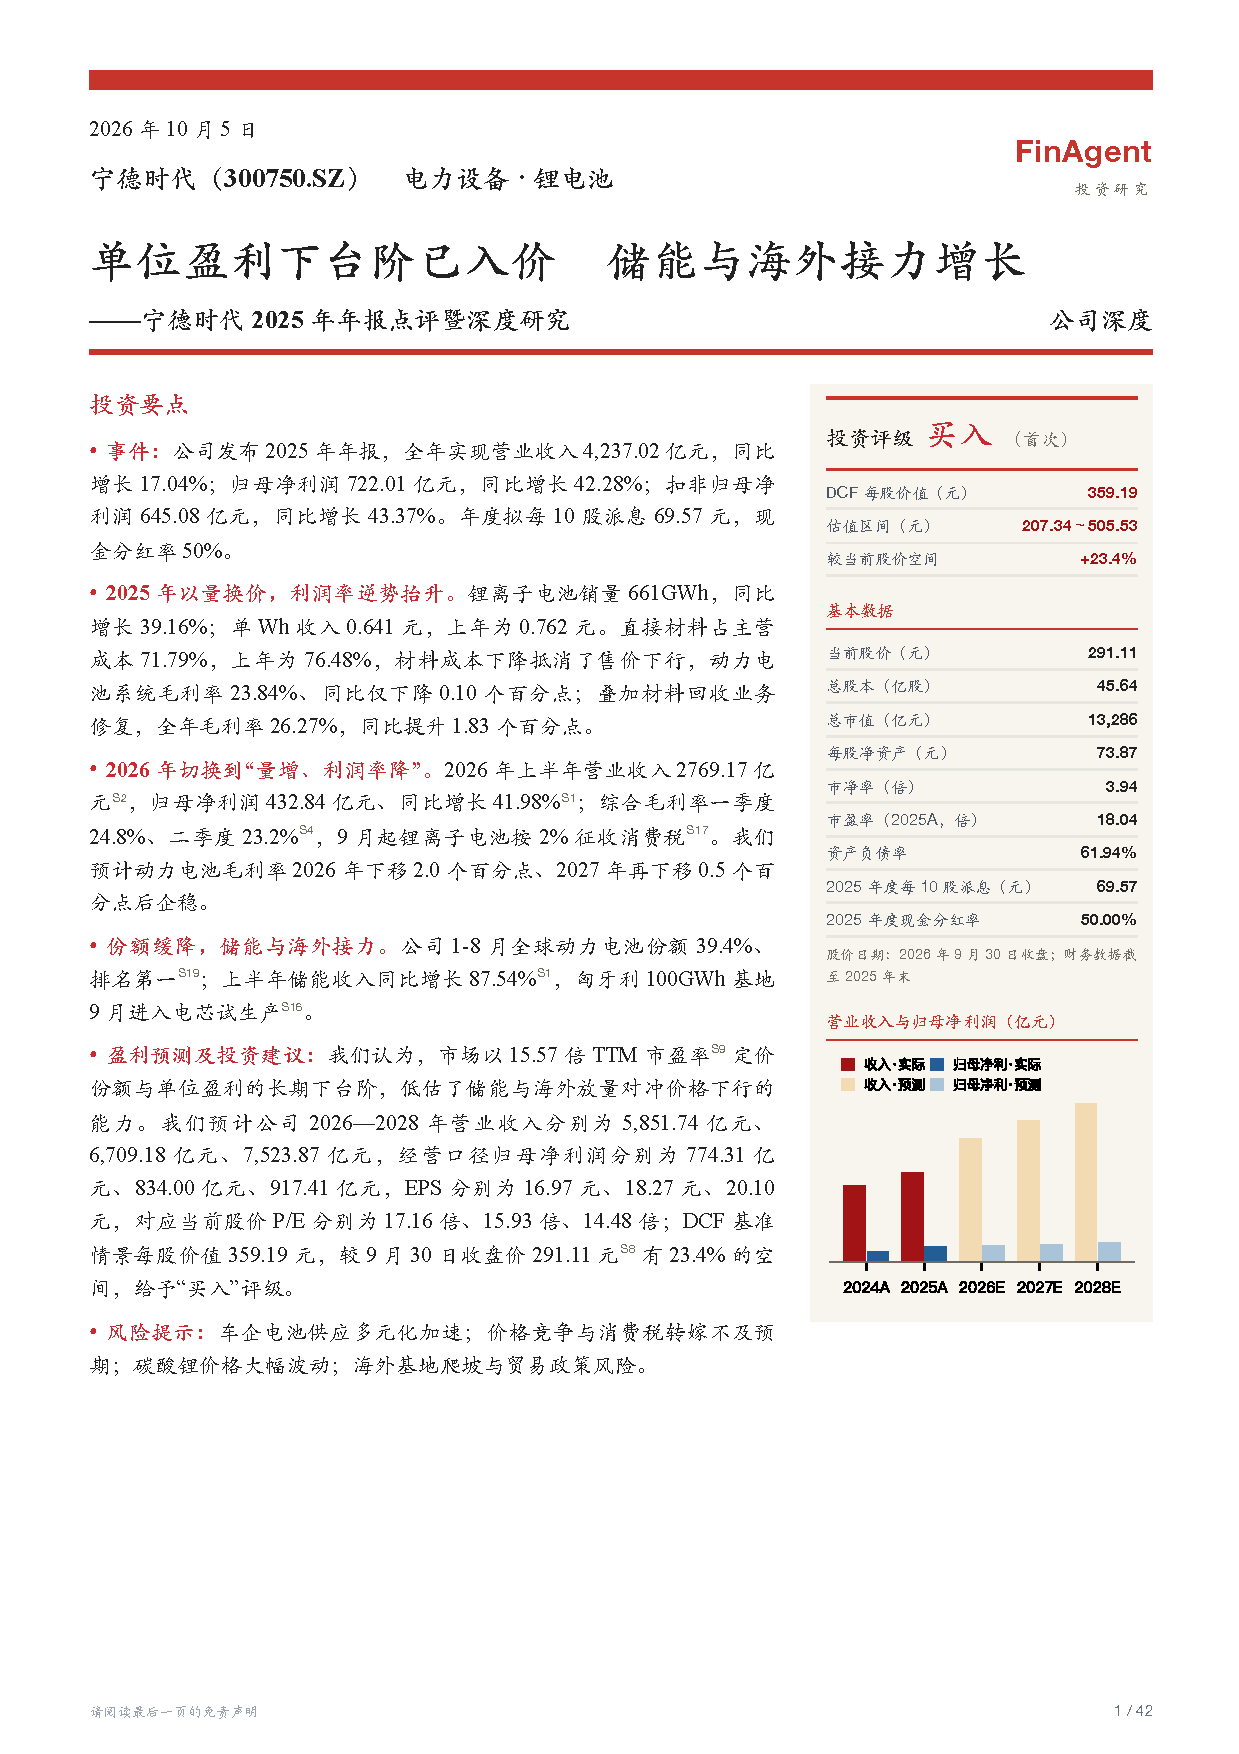
\includepdf[pages=-,scale=0.86,frame,pagecommand={\thispagestyle{fancy}}]{figures/report_catl.pdf}


\end{document}
